\chapter{Vi phân tự động và các thuật toán tối ưu}
\label{chap:autodiff}
 
Chương~\ref{chap:fnn} đã mô tả mạng nơ-ron truyền thẳng như một họ hàm tham số
hoá $\Net_{\btheta}$ có khả năng xấp xỉ phổ quát theo chuẩn $C^k$
(Định lý~\ref{dl:sobolev}). Nhưng một định lý xấp xỉ chỉ khẳng định \emph{sự tồn
tại} của bộ tham số tốt; nó không cho biết cách tìm ra bộ tham số đó, và
Mệnh đề~\ref{md:khong-loi} đã cho thấy không thể trông đợi một bảo đảm hội tụ
toàn cục nào. Toàn bộ khoảng cách giữa khả năng biểu diễn lý thuyết và một
nghiệm số dùng được nằm ở hai công cụ được trình bày trong chương này.
 
Công cụ thứ nhất là \emph{vi phân tự động}: một cơ chế tính đạo hàm chính xác
tới độ chính xác máy với chi phí chỉ bằng một bội số nhỏ của chi phí đánh giá
hàm, và -- điểm quyết định đối với báo cáo -- áp dụng được \emph{đệ quy lên
chính nó} để thu được đạo hàm bậc cao theo biến đầu vào. Công cụ thứ hai là
\emph{các thuật toán tối ưu} bậc nhất và tựa Newton, cho phép cực tiểu hoá hàm
mục tiêu trên không gian tham số nhiều chiều.
 
Sự phân biệt giữa hai loại đạo hàm cần được nhắc lại, vì nó là trục của chương.
Trong mạng nơ-ron thông thường, ta chỉ cần $\nabla_{\btheta} J$ để huấn luyện.
Khi giải phương trình vi phân, ta còn cần $\partial_{\bx}\Net_{\btheta}$ và
$\nabla^2_{\bx}\Net_{\btheta}$ để dựng phần dư, rồi lại lấy đạo hàm của phần dư
đó theo $\btheta$. Chương~\ref{chap:fnn} đã cho công thức truy hồi tường minh cho
hai đại lượng đầu (Mệnh đề~\ref{md:jacobian} và Mệnh đề~\ref{md:hessian}); mục
tiêu của Mục~\ref{subsec:bac-cao-ad} là chỉ ra rằng vi phân tự động tính đúng các
đại lượng ấy mà không cần lập trình tường minh $\sigma''$, và giải thích cái giá
phải trả về bộ nhớ.
 
\subsubsection*{Quy ước ký hiệu bổ sung}
 
Chương này giữ nguyên toàn bộ ký hiệu của Bảng~\ref{tab:ky-hieu}, đặc biệt là
quy ước lớp ra tuyến tính $\Net_{\btheta}(\bx) = \bz^{(L)}$ của
Định nghĩa~\ref{def:fnn}. Ba ký hiệu mới được thêm:
 
\begin{itemize}[leftmargin=*]
\item $\varrho(\hat{\bm{y}}, \bm{y})$ -- hàm mất mát \emph{tại một điểm}. Ta
      không dùng ký hiệu $\mathcal{L}$ cho đại lượng này, vì $\mathcal{L}$ được
      dành riêng cho toán tử vi phân trong toàn bộ báo cáo.
\item $\D f(\bx) \in \R^{m\times n}$ -- ma trận Jacobi của
      $f:\R^n\to\R^m$ tại $\bx$. Ta không dùng $\bm{J}_f$ để tránh nhầm với hàm
      mục tiêu $J$.
\item $\eps \approx 2{,}22\times 10^{-16}$ -- epsilon máy của số thực dấu phẩy
      động độ chính xác kép.
\end{itemize}
 
%==============================================================================
\section{Lan truyền ngược}
\label{sec:backprop}
%==============================================================================
 
\subsection{Bài toán tính gradient}
\label{subsec:bai-toan-gradient}
 
Việc huấn luyện là bài toán cực tiểu hoá không ràng buộc
\begin{equation}
\min_{\btheta \in \R^P} \; J(\btheta),
\qquad
J(\btheta) = \frac{1}{N}\sum_{i=1}^{N}
  \varrho\!\left( \Net_{\btheta}(\bx_i),\, \bm{y}_i \right),
\label{eq:erm}
\end{equation}
với $P$ cho bởi \eqref{eq:so-tham-so}. Mọi thuật toán ở Mục~\ref{sec:optimizers}
đều cần vectơ gradient $\nabla_{\btheta} J \in \R^P$. Vì $P$ thường nằm trong
khoảng $10^3$ đến $10^7$, câu hỏi cốt lõi không phải là ``tính được hay không''
mà là: \emph{chi phí tính $\nabla_{\btheta} J$ phụ thuộc thế nào vào $P$?}
 
Câu trả lời ngây thơ -- xấp xỉ từng đạo hàm riêng bằng sai phân hữu hạn -- đòi
hỏi ít nhất $2P$ lần lan truyền xuôi cho công thức trung tâm, và cho kết quả chỉ
chính xác vài chữ số (Mục~\ref{subsec:fd-fail}). Lan truyền ngược cho một câu trả
lời tốt hơn hẳn về cả hai phương diện: \emph{toàn bộ} gradient được tính chính
xác tới độ chính xác máy, với chi phí chỉ khoảng hai đến ba lần một lượt lan
truyền xuôi, \emph{độc lập với $P$}.
 
\subsection{Đồ thị tính toán}
\label{subsec:comp-graph}
 
\begin{definition}[Đồ thị tính toán]
\label{def:comp-graph}
\emph{Đồ thị tính toán} của một biểu thức là một đồ thị có hướng không chu trình
$G = (V,E)$, trong đó mỗi đỉnh $v \in V$ tương ứng với một biến trung gian, mỗi
đỉnh không phải đỉnh nguồn được gán một phép toán sơ cấp $\varphi_v$, và cung
$(u,v) \in E$ tồn tại khi và chỉ khi biến $u$ là đối số trực tiếp của
$\varphi_v$. Ta ký hiệu $\mathrm{Pa}(v)$ là tập đỉnh cha (đối số) và
$\mathrm{Ch}(v)$ là tập đỉnh con (các đỉnh nhận $v$ làm đối số) của $v$.
\end{definition}
 
Cách nhìn này, được nhấn mạnh ở Mục 6.5 của Goodfellow và cộng
sự~\cite{goodfellow2016} và được Hammad~\cite{hammad2024} minh hoạ bằng các ví
dụ tính tay, tách bạch \emph{cấu trúc} của phép tính đạo hàm khỏi \emph{nội
dung} cụ thể của mô hình. Hệ thức truy hồi
\eqref{eq:fnn-affine}--\eqref{eq:fnn-act} chỉ là một đồ thị tính toán đặc biệt có
dạng chuỗi; hoàn toàn có thể thay nó bằng mạng có kết nối tắt, mạng tuần hoàn,
hay biểu thức phần dư của một phương trình vi phân, mà cơ chế lấy đạo hàm không
thay đổi một dòng nào. Chính tính bất biến này là điều làm cho vi phân tự động
trở thành công cụ đúng cho bài toán của báo cáo: phần dư
$\mathcal{L}[\Net_{\btheta}] - f$ cũng chỉ là một đỉnh khác trong cùng đồ thị.
 
\begin{figure}[htbp]
\centering
\begin{tikzpicture}[
  >={Stealth[round]},
  node distance = 9mm and 13mm,
  op/.style   = {draw, rounded corners=2pt, minimum height=7mm,
                 minimum width=9mm, font=\small, inner sep=3pt},
  var/.style  = {draw, circle, minimum size=7mm, font=\small, inner sep=1pt},
  every path/.style = {->, thick}
]
\node[var] (x)  {$\bx$};
\node[op, right=of x]   (z1) {$\bz^{(1)}$};
\node[op, right=of z1]  (a1) {$\ba^{(1)}$};
\node[op, right=of a1]  (z2) {$\bz^{(2)}$};
\node[op, right=of z2]  (J)  {$J$};
 
\node[var, above=of z1] (W1) {$\bW^{(1)}$};
\node[var, below=of z1] (b1) {$\bb^{(1)}$};
\node[var, above=of z2] (W2) {$\bW^{(2)}$};
\node[var, below=of z2] (b2) {$\bb^{(2)}$};
\node[var, above=of J]  (y)  {$\bm{y}$};
 
\draw (x)  -- (z1);
\draw (W1) -- (z1);
\draw (b1) -- (z1);
\draw (z1) -- node[above, font=\scriptsize] {$\sigma$} (a1);
\draw (a1) -- (z2);
\draw (W2) -- (z2);
\draw (b2) -- (z2);
\draw (z2) -- node[above, font=\scriptsize] {$\varrho$} (J);
\draw (y)  -- (J);
\end{tikzpicture}
\caption{Đồ thị tính toán của một mạng truyền thẳng $L = 2$ cùng hàm mất mát.
Lớp ra tuyến tính theo quy ước \eqref{eq:fnn-output}, nên $\bz^{(2)}$ đi thẳng
vào $\varrho$ mà không qua $\sigma$. Lượt xuôi đi theo chiều cung; lan truyền
ngược đi ngược chiều cung, tích luỹ tại mỗi đỉnh đại lượng liên hợp
$\partial J/\partial v$.}
\label{fig:comp-graph}
\end{figure}
 
\subsection{Quy tắc dây chuyền trên đồ thị và tích vectơ--Jacobi}
\label{subsec:vjp}
 
Xét một đỉnh $v$ trong đồ thị. Vì $J$ phụ thuộc vào $v$ chỉ thông qua các đỉnh
con trực tiếp của nó, quy tắc dây chuyền nhiều biến cho
\begin{equation}
\frac{\partial J}{\partial v}
= \sum_{w \in \mathrm{Ch}(v)}
\left( \frac{\partial w}{\partial v} \right)^{\!\top}
\frac{\partial J}{\partial w}.
\label{eq:chain-graph}
\end{equation}
Đây chính là toàn bộ nội dung của lan truyền ngược: duyệt đồ thị theo thứ tự
tô-pô ngược và áp dụng \eqref{eq:chain-graph} tại từng đỉnh. Mọi thứ còn lại
trong mục này là hệ quả của \eqref{eq:chain-graph} áp cho cấu trúc chuỗi cụ thể.
 
Cần nhấn mạnh một điểm về cài đặt mà \eqref{eq:chain-graph} che giấu. Đại lượng
$\partial w/\partial v$ là một \emph{ma trận Jacobi}, và điều thực sự được thực
hiện trên máy không phải là dựng ma trận đó rồi nhân, mà là tính trực tiếp
\emph{tích vectơ--Jacobi} (vector--Jacobian product, VJP)
\begin{equation}
\bar{\bm{w}} \;\longmapsto\; \bar{\bm{w}}^{\top}\, \D\varphi_w(v)
\label{eq:vjp}
\end{equation}
với chi phí bằng đúng bậc chi phí đánh giá phép toán $\varphi_w$. Sự phân biệt
này không phải chi tiết kỹ thuật: Jacobi của một lớp có $n_\ell n_{\ell-1} =
10^6$ phần tử là bất khả thi về bộ nhớ nếu dựng tường minh, trong khi VJP của
cùng lớp ấy chỉ là một phép nhân với ma trận chuyển vị.
 
\subsection{Bốn phương trình của lan truyền ngược}
\label{subsec:bon-pt}

Bốn hệ thức dưới đây là dạng ma trận của thuật toán lan truyền ngược; cách trình
bày qua đồ thị tính toán ở đây theo Goodfellow và cộng sự~\cite{goodfellow2016},
còn ký hiệu $\bm{\delta}^{(\ell)}$ thì bám theo quy ước đã dùng từ
Chương~\ref{chap:fnn}.

Áp dụng \eqref{eq:chain-graph} cho cấu trúc chuỗi
\eqref{eq:fnn-input}--\eqref{eq:fnn-output}, ta thu được dạng ma trận. Đặt
\emph{sai số cục bộ} (local error, hay biến liên hợp) của lớp $\ell$ là
\begin{equation}
\bm{\delta}^{(\ell)} \coloneqq \frac{\partial J}{\partial \bz^{(\ell)}}
\in \R^{n_\ell},
\label{eq:delta-def}
\end{equation}
đúng như ký hiệu đã dùng ở Mệnh đề~\ref{md:tich-gradient} và
Mệnh đề~\ref{md:var-nguoc}.
 
\begin{menhde}[Các phương trình lan truyền ngược]
\label{md:bp}
Với mạng theo Định nghĩa~\ref{def:fnn} (lớp ra tuyến tính), $\sigma \in C^1$ và
hàm mất mát $J$ khả vi, ta có
\begin{align}
\bm{\delta}^{(L)} &= \nabla_{\bz^{(L)}} J
  \;=\; \nabla_{\Net_{\btheta}} J,
\label{eq:bp1}\\[2pt]
\bm{\delta}^{(\ell)} &= \left[ \left(\bW^{(\ell+1)}\right)^{\!\top}
  \bm{\delta}^{(\ell+1)} \right]
\odot \sigma'\!\left(\bz^{(\ell)}\right),
\qquad \ell = L-1,\dots,1,
\label{eq:bp2}\\[2pt]
\frac{\partial J}{\partial \bW^{(\ell)}}
  &= \bm{\delta}^{(\ell)} \left(\ba^{(\ell-1)}\right)^{\!\top},
\label{eq:bp3}\\[2pt]
\frac{\partial J}{\partial \bb^{(\ell)}} &= \bm{\delta}^{(\ell)},
\label{eq:bp4}
\end{align}
trong đó $\odot$ là tích Hadamard (nhân theo từng thành phần). Dạng
\eqref{eq:bp2} tương đương với dạng ma trận
$\bm{\delta}^{(\ell)} = \bD^{(\ell)}\big(\bW^{(\ell+1)}\big)^{\!\top}
\bm{\delta}^{(\ell+1)}$ đã dùng ở Chương~\ref{chap:fnn}, với
$\bD^{(\ell)} = \diag\!\big(\sigma'(\bz^{(\ell)})\big)$.
\end{menhde}
 
\begin{proof}
Với \eqref{eq:bp1}: theo \eqref{eq:fnn-output}, $\Net_{\btheta} = \bz^{(L)}$,
nên hai gradient trùng nhau theo định nghĩa. (Nếu lớp ra có kích hoạt
$\sigma^{(L)}$, công thức trở thành
$\bm{\delta}^{(L)} = \nabla_{\ba^{(L)}}J \odot \sigma'^{(L)}(\bz^{(L)})$; ta nêu
để đối chiếu, nhưng báo cáo không dùng trường hợp này.)
 
Với \eqref{eq:bp2}: biến $z^{(\ell)}_j$ ảnh hưởng đến $J$ chỉ thông qua toàn bộ
các biến $z^{(\ell+1)}_k$, $k = 1,\dots,n_{\ell+1}$. Từ \eqref{eq:z-k},
\[
z^{(\ell+1)}_k = \sum_{j} w^{(\ell+1)}_{kj}\,
  \sigma\!\left(z^{(\ell)}_j\right) + b^{(\ell+1)}_k
\quad\Longrightarrow\quad
\frac{\partial z^{(\ell+1)}_k}{\partial z^{(\ell)}_j}
= w^{(\ell+1)}_{kj}\, \sigma'\!\left(z^{(\ell)}_j\right),
\]
trong đó ta đã dùng việc $\sigma$ tác động theo từng thành phần: $z^{(\ell)}_j$
chỉ ảnh hưởng tới $a^{(\ell)}_j$, không ảnh hưởng tới $a^{(\ell)}_{j'}$ với
$j'\ne j$. Thay vào \eqref{eq:chain-graph}:
\[
\delta^{(\ell)}_j
= \sum_{k=1}^{n_{\ell+1}} \delta^{(\ell+1)}_k\, w^{(\ell+1)}_{kj}\,
  \sigma'\!\left(z^{(\ell)}_j\right)
= \left[ \left(\bW^{(\ell+1)}\right)^{\!\top}\bm{\delta}^{(\ell+1)} \right]_j
  \sigma'\!\left(z^{(\ell)}_j\right).
\]
Vì $\sigma'(z^{(\ell)}_j)$ chỉ nhân vào thành phần thứ $j$, phép nhân này đúng
là tích Hadamard, và cũng đúng là phép nhân trái với ma trận đường chéo
$\bD^{(\ell)}$.
 
Với \eqref{eq:bp3}--\eqref{eq:bp4}: từ \eqref{eq:z-k},
$\partial z^{(\ell)}_j/\partial w^{(\ell)}_{pq} = \delta_{jp}\, a^{(\ell-1)}_q$
và $\partial z^{(\ell)}_j/\partial b^{(\ell)}_p = \delta_{jp}$, với $\delta_{jp}$
là ký hiệu Kronecker. Do đó
\[
\frac{\partial J}{\partial w^{(\ell)}_{pq}}
= \sum_j \delta^{(\ell)}_j\, \delta_{jp}\, a^{(\ell-1)}_q
= \delta^{(\ell)}_p\, a^{(\ell-1)}_q,
\qquad
\frac{\partial J}{\partial b^{(\ell)}_p} = \delta^{(\ell)}_p . \qedhere
\]
\end{proof}
 
\begin{nhanxet}
\label{nx:bp-structure}
Ba đặc điểm cấu trúc đáng chú ý, mỗi đặc điểm nối với một kết quả đã có.
 
\emph{(a) Tích ngoài và chi phí bộ nhớ.} Công thức \eqref{eq:bp3} có dạng tích
ngoài: gradient đối với ma trận trọng số là tích của tín hiệu lỗi đi ngược với
tín hiệu kích hoạt đi xuôi. Đây là lý do buộc phải \emph{lưu lại} các
$\ba^{(\ell-1)}$ trong lượt xuôi, và là nguồn gốc của chi phí bộ nhớ
$\mathcal{O}(N\sum_\ell n_\ell)$ đã nêu ở Mệnh đề~\ref{md:chi-phi}.
 
\emph{(b) Tích các $\sigma'$.} Thừa số $\sigma'(\bz^{(\ell)})$ xuất hiện trong
mọi bước lùi. Tích luỹ qua $L$ lớp, nó sinh ra đúng tích ma trận đã được chặn ở
Mệnh đề~\ref{md:tich-gradient}, và chính tích này gây hiện tượng triệt tiêu hoặc
bùng nổ gradient.
 
\emph{(c) Trường hợp của báo cáo.} Với lớp ra tuyến tính và
$\varrho(\hat{\bm y},\bm y) = \tfrac12\|\hat{\bm y}-\bm y\|_2^2$,
\eqref{eq:bp1} rút gọn thành $\bm{\delta}^{(L)} = \Net_{\btheta}(\bx) - \bm{y}$,
tức đúng bằng phần dư của phép khớp. Trong bài toán PINN, vai trò của
$\bm y$ được thay bằng vế phải của phương trình và $\Net_{\btheta}$ được thay
bằng $\mathcal{L}[\Net_{\btheta}]$; cấu trúc của \eqref{eq:bp1} không đổi, chỉ
có đồ thị phía trước nó dài hơn.
\end{nhanxet}
 
\paragraph{Dạng theo lô.} Với lô $N$ mẫu và ký hiệu ma trận
$\bm{A}^{(\ell)}, \bm{Z}^{(\ell)}$ của \eqref{eq:batch}, đặt
$\bm{\Delta}^{(\ell)} = \big[\bm{\delta}^{(\ell)}_1,\dots,
\bm{\delta}^{(\ell)}_N\big] \in \R^{n_\ell\times N}$. Khi ấy
\eqref{eq:bp2}--\eqref{eq:bp4} trở thành
\begin{equation}
\begin{aligned}
\bm{\Delta}^{(\ell)} &= \left[\left(\bW^{(\ell+1)}\right)^{\!\top}
  \bm{\Delta}^{(\ell+1)}\right] \odot \sigma'\!\left(\bm{Z}^{(\ell)}\right),\\
\frac{\partial J}{\partial \bW^{(\ell)}}
 &= \frac{1}{N}\,\bm{\Delta}^{(\ell)}\big(\bm{A}^{(\ell-1)}\big)^{\!\top},
\qquad
\frac{\partial J}{\partial \bb^{(\ell)}}
 = \frac{1}{N}\,\bm{\Delta}^{(\ell)}\bm{1}_N .
\end{aligned}
\label{eq:bp-batch}
\end{equation}
Phép lấy tổng theo mẫu, vốn là một vòng lặp trong dạng \eqref{eq:bp3}, đã được
thu vào \emph{một} phép nhân ma trận. Đây là lý do kỹ thuật khiến huấn luyện theo
lô nhanh hơn nhiều lần so với xử lý từng mẫu, dù tổng số phép toán số thực là như
nhau.
 
\begin{algorithm}[htbp]
\caption{Lan truyền ngược cho mạng truyền thẳng $L$ lớp}
\label{alg:backprop}
\begin{algorithmic}[1]
\Require Đầu vào $\bx$, nhãn $\bm{y}$, tham số
  $\{\bW^{(\ell)},\bb^{(\ell)}\}_{\ell=1}^{L}$
\Ensure Gradient $\{\partial J/\partial \bW^{(\ell)},\,
  \partial J/\partial \bb^{(\ell)}\}_{\ell=1}^{L}$
\State $\ba^{(0)} \gets \bx$
\For{$\ell = 1$ \textbf{đến} $L$} \Comment{lượt xuôi, Thuật toán~\ref{alg:forward}}
  \State $\bz^{(\ell)} \gets \bW^{(\ell)}\ba^{(\ell-1)} + \bb^{(\ell)}$
  \State \textbf{nếu} $\ell < L$ \textbf{thì} $\ba^{(\ell)} \gets
    \sigma(\bz^{(\ell)})$ \textbf{ngược lại} $\ba^{(L)} \gets \bz^{(L)}$
  \State lưu $\ba^{(\ell-1)}$ và $\bz^{(\ell)}$ vào băng ghi
\EndFor
\State $\bm{\delta}^{(L)} \gets \nabla_{\bz^{(L)}} J$
  \Comment{\eqref{eq:bp1}}
\For{$\ell = L$ \textbf{xuống} $1$} \Comment{lượt ngược}
  \State $\partial J/\partial \bW^{(\ell)} \gets
    \bm{\delta}^{(\ell)}\big(\ba^{(\ell-1)}\big)^{\!\top}$
    \Comment{\eqref{eq:bp3}}
  \State $\partial J/\partial \bb^{(\ell)} \gets \bm{\delta}^{(\ell)}$
    \Comment{\eqref{eq:bp4}}
  \If{$\ell > 1$}
    \State $\bm{\delta}^{(\ell-1)} \gets
      \left[\big(\bW^{(\ell)}\big)^{\!\top}\bm{\delta}^{(\ell)}\right]
      \odot \sigma'\!\left(\bz^{(\ell-1)}\right)$
      \Comment{\eqref{eq:bp2}}
  \EndIf
\EndFor
\end{algorithmic}
\end{algorithm}
 
\subsection{Chi phí tính toán}
\label{subsec:chi-phi-bp}
 
\begin{menhde}[Chi phí của lan truyền ngược]
\label{md:chi-phi-bp}
Với mạng theo Định nghĩa~\ref{def:fnn} và lô $N$ mẫu, lượt ngược của
Thuật toán~\ref{alg:backprop} tiêu tốn
\begin{equation}
B = 4N\sum_{\ell=1}^{L} n_\ell n_{\ell-1}
  \;-\; 2N\, n_L n_{L-1}
\label{eq:bp-cost-exact}
\end{equation}
phép toán số thực, tức
$\mathrm{cost}\big(\nabla_{\btheta} J\big) \le c\cdot
\mathrm{cost}\big(J\big)$ với $c \le 3$, \emph{độc lập với số tham số $P$}, trong
đó $\mathrm{cost}(J)$ là chi phí \eqref{eq:do-phuc-tap} của lượt xuôi.
\end{menhde}
 
\begin{proof}
Ở lớp $\ell$, lượt ngược thực hiện hai phép toán có bậc $n_\ell n_{\ell-1}$.
 
Thứ nhất, tích ngoài \eqref{eq:bp3}: ma trận kết quả có $n_\ell n_{\ell-1}$ phần
tử, mỗi phần tử là một phép nhân, cộng thêm phép cộng tích luỹ theo $N$ mẫu
trong dạng \eqref{eq:bp-batch}, tổng cộng $2N n_\ell n_{\ell-1}$ phép.
 
Thứ hai, phép nhân với ma trận chuyển vị trong \eqref{eq:bp2}: theo cùng lập luận
đếm của Mệnh đề~\ref{md:chi-phi}, phép này tốn $2N n_\ell n_{\ell-1}$ phép. Phép
này không được thực hiện tại lớp cuối ($\ell = L$ chỉ cần \eqref{eq:bp1}), từ đó
có số hạng trừ trong \eqref{eq:bp-cost-exact}. Phép nhân Hadamard với
$\sigma'(\bz^{(\ell)})$ chỉ tốn $N n_\ell$ phép, thuộc bậc thấp hơn.
 
Chia \eqref{eq:bp-cost-exact} cho \eqref{eq:do-phuc-tap} được tỉ số không vượt
quá $2$; cộng thêm chính lượt xuôi (bắt buộc phải chạy trước) cho $c \le 3$. Mọi
đại lượng trong lập luận chỉ phụ thuộc kiến trúc, không phụ thuộc $P$ theo bất kỳ
cách nào khác ngoài qua chính tổng $\sum_\ell n_\ell n_{\ell-1}$ vốn đã có mặt
trong $\mathrm{cost}(J)$.
\end{proof}
 
So sánh với chi phí $\mathcal{O}(P)\cdot\mathrm{cost}(J)$ của sai phân hữu hạn,
đây là mức chênh lệch nhiều bậc độ lớn: với $P = 10^4$, lan truyền ngược nhanh
hơn khoảng ba nghìn lần. Đây là lý do kỹ thuật khiến mạng nơ-ron sâu trở nên khả
thi. Cái giá phải trả là bộ nhớ: băng ghi phải giữ toàn bộ giá trị trung gian của
lượt xuôi cho tới khi lượt ngược dùng đến chúng. Sự đánh đổi thời gian--bộ nhớ
này sẽ trở nên gay gắt hơn nhiều ở Mục~\ref{subsec:bac-cao-ad}, khi ta lấy đạo
hàm bậc hai.
 
\subsection{Ví dụ tính toán chi tiết}
\label{subsec:vd-backprop}
 
\begin{vidu}
\label{vd:backprop-numeric}
Xét mạng $(1,2,1)$ với $\sigma = \tanh$ ở lớp ẩn, lớp ra tuyến tính, và
$\varrho(\hat y, y) = \tfrac{1}{2}(\hat{y}-y)^2$. Cho
\[
\bW^{(1)} = \begin{pmatrix} 0{,}5 \\ -0{,}3 \end{pmatrix},\quad
\bb^{(1)} = \begin{pmatrix} 0{,}1 \\ 0{,}2 \end{pmatrix},\quad
\bW^{(2)} = \begin{pmatrix} 0{,}4 & 0{,}7 \end{pmatrix},\quad
b^{(2)} = -0{,}1,
\]
với mẫu dữ liệu $x = 1$, $y = 0{,}5$.
 
\smallskip
\noindent\textbf{Lượt xuôi.} Theo \eqref{eq:z-k},
\[
\bz^{(1)} = \begin{pmatrix} 0{,}6 \\ -0{,}1 \end{pmatrix},
\qquad
\ba^{(1)} = \tanh\!\left(\bz^{(1)}\right)
= \begin{pmatrix} 0{,}537050 \\ -0{,}099668 \end{pmatrix},
\]
\begin{gather*}
\hat{y} = z^{(2)} = 0{,}4 \cdot 0{,}537050 + 0{,}7 \cdot (-0{,}099668) - 0{,}1
 = 0{,}045052, \\
J = \tfrac{1}{2}\big(0{,}045052 - 0{,}5\big)^2 = 0{,}103489 .
\end{gather*}
 
\noindent\textbf{Lượt ngược.} Vì lớp ra tuyến tính, \eqref{eq:bp1} cho
\[
\delta^{(2)} = \hat{y} - y = -0{,}454948 .
\]
Từ \eqref{eq:bp3}--\eqref{eq:bp4},
\[
\frac{\partial J}{\partial \bW^{(2)}}
= \delta^{(2)} \left(\ba^{(1)}\right)^{\!\top}
= \begin{pmatrix} -0{,}244330 & 0{,}045344 \end{pmatrix},
\qquad
\frac{\partial J}{\partial b^{(2)}} = -0{,}454948 .
\]
Dùng \eqref{eq:tanh-d1}, tức $\tanh'(z) = 1 - \tanh^2 z$, ta có
$\sigma'(\bz^{(1)}) = (0{,}711578;\; 0{,}990066)^{\top}$, và \eqref{eq:bp2} cho
\[
\begin{aligned}
\bm{\delta}^{(1)}
&= \left[\left(\bW^{(2)}\right)^{\!\top}\delta^{(2)}\right]
   \odot \sigma'\!\left(\bz^{(1)}\right) \\[2pt]
&= \begin{pmatrix} -0{,}181979 \\ -0{,}318463 \end{pmatrix}
   \odot
   \begin{pmatrix} 0{,}711578 \\ 0{,}990066 \end{pmatrix}
 = \begin{pmatrix} -0{,}129492 \\ -0{,}315300 \end{pmatrix}.
\end{aligned}
\]
Cuối cùng, do $a^{(0)} = x = 1$, hai công thức
\eqref{eq:bp3}--\eqref{eq:bp4} trùng nhau:
\[
\frac{\partial J}{\partial \bW^{(1)}}
= \frac{\partial J}{\partial \bb^{(1)}}
= \begin{pmatrix} -0{,}129492 \\ -0{,}315300 \end{pmatrix}.
\]
 
\noindent\textbf{Kiểm chứng.} Sai phân trung tâm với $h = 10^{-6}$ đối với thành
phần $w^{(1)}_{11}$ cho $-0{,}1294922863$, trùng với kết quả giải tích tới chữ
số có nghĩa thứ tám. Cần đọc kết quả này cho đúng: tám chữ số là mức chính xác
\emph{tối đa} mà sai phân hữu hạn đạt được ở đây, trong khi lan truyền ngược cho
kết quả chính xác tới độ chính xác máy. Mục~\ref{subsec:fd-fail} lượng hoá chính
xác rào cản này.
\end{vidu}
 
%==============================================================================
\section{Vi phân tự động}
\label{sec:ad}
%==============================================================================
 
\subsection{Bốn cách tính đạo hàm}
\label{subsec:bon-cach}
 
Trước khi định nghĩa vi phân tự động, cần phân biệt rõ nó với ba cách tiếp cận
khác thường bị nhầm lẫn~\cite{baydin2018}.
 
\emph{Vi phân thủ công.} Người dùng tự lấy đạo hàm bằng tay rồi lập trình công
thức thu được -- đúng như Ví dụ~\ref{vd:backprop-numeric} vừa làm. Chính xác
nhưng tốn công, dễ sai, và phải làm lại mỗi khi đổi kiến trúc mô hình hoặc đổi
phương trình.
 
\emph{Vi phân ký hiệu} (symbolic). Hệ thống đại số máy tính biến đổi biểu thức
thành biểu thức đạo hàm. Chính xác, nhưng gặp hiện tượng \emph{bùng nổ biểu
thức}: đạo hàm của một hàm hợp $L$ tầng có thể dài theo hàm mũ theo $L$ nếu các
biểu thức con không được chia sẻ. Hệ truy hồi \eqref{eq:S-truy-hoi} cho một ví dụ
cụ thể: khai triển hoàn toàn $\bS^{(\ell)}_k$ theo các trọng số sinh ra một tổng
có số hạng tăng theo $\prod_\ell n_\ell$.
 
\emph{Vi phân số} (sai phân hữu hạn). Xấp xỉ
\begin{equation}
\frac{\partial f}{\partial x_i}(\bx)
\approx \frac{f(\bx+h\bm{e}_i) - f(\bx-h\bm{e}_i)}{2h}.
\label{eq:fd}
\end{equation}
Đơn giản, không xâm lấn mã nguồn, nhưng có hai khuyết điểm chí mạng được phân
tích ngay dưới đây.
 
\emph{Vi phân tự động}. Không thao tác trên biểu thức mà trên \emph{chương
trình}: mọi hàm khả vi được cài trên máy đều là hợp của một tập hữu hạn phép toán
sơ cấp có đạo hàm đã biết; vi phân tự động áp dụng quy tắc dây chuyền một cách hệ
thống lên dãy phép toán đó. Kết quả \emph{chính xác} -- không có sai số cắt cụt,
chỉ có sai số làm tròn thông thường của chính phép đánh giá hàm -- và chi phí bị
chặn bởi một bội số nhỏ của chi phí đánh giá hàm.
 
\subsection{Vì sao sai phân hữu hạn không đủ}
\label{subsec:fd-fail}
 
\begin{menhde}[Rào cản độ chính xác của sai phân trung tâm]
\label{md:fd-rao-can}
Giả sử $f \in C^3$ trong lân cận của $\bx$ và các giá trị $f(\bx\pm h\bm{e}_i)$
được tính với sai số tương đối cỡ $\eps$. Khi đó sai số của
\eqref{eq:fd} bị chặn bởi
\begin{equation}
E(h) \;\le\; \underbrace{C_1 h^2}_{\text{cắt cụt}}
 \;+\; \underbrace{\frac{C_2\,\eps}{h}}_{\text{làm tròn}},
\qquad
C_1 = \frac{1}{6}\sup\big|\partial_i^3 f\big|,
\quad
C_2 = \sup|f| ,
\label{eq:fd-sai-so}
\end{equation}
và vế phải đạt cực tiểu tại
\begin{equation}
h^{*} = \left(\frac{C_2\,\eps}{2C_1}\right)^{1/3},
\qquad
E(h^{*}) = 3\left(\frac{C_1 C_2^2}{4}\right)^{1/3} \eps^{2/3}.
\label{eq:fd-toi-uu}
\end{equation}
\end{menhde}
 
\begin{proof}
Khai triển Taylor tới bậc ba quanh $\bx$:
$f(\bx\pm h\bm{e}_i) = f \pm h\partial_i f + \tfrac{h^2}{2}\partial_i^2 f
\pm \tfrac{h^3}{6}\partial_i^3 f(\bm{\xi}_\pm)$. Lấy hiệu và chia $2h$, các số
hạng bậc chẵn triệt tiêu, còn lại sai số cắt cụt bị chặn bởi
$\tfrac{h^2}{6}\sup|\partial_i^3 f| = C_1h^2$.
 
Về sai số làm tròn: mỗi giá trị $f(\bx\pm h\bm{e}_i)$ được lưu với sai số tuyệt
đối cỡ $\eps|f|$. Hiệu của chúng do đó mang sai số cỡ $2\eps|f|$, và sau khi chia
cho $2h$ ta được $\eps|f|/h \le C_2\eps/h$. Cộng hai nguồn cho
\eqref{eq:fd-sai-so}.
 
Cực tiểu hoá $g(h) = C_1h^2 + C_2\eps/h$ trên $(0,\infty)$: $g'(h) = 2C_1 h -
C_2\eps/h^2 = 0$ cho $h^3 = C_2\eps/(2C_1)$, tức $h^*$ như trong
\eqref{eq:fd-toi-uu}; vì $g'' > 0$ đây là cực tiểu. Thay vào:
$g(h^*) = C_1 h^{*2} + C_2\eps/h^* = 3C_1h^{*2}$ (dùng
$C_2\eps = 2C_1h^{*3}$), và khai triển $h^{*2}$ cho biểu thức đã nêu.
\end{proof}
 
\begin{nhanxet}[Đọc \eqref{eq:fd-toi-uu} cho đúng]
\label{nx:fd-hang-so}
Với $C_1, C_2$ cỡ đơn vị, \eqref{eq:fd-toi-uu} cho các con số thường được trích
dẫn: $h^{*} \sim \eps^{1/3} \approx 6\times 10^{-6}$ và sai số tốt nhất
$\sim \eps^{2/3} \approx 3{,}7\times 10^{-11}$. Nhưng \emph{hai hằng số này phụ
thuộc bài toán}, và bỏ qua chúng dẫn tới mâu thuẫn với số liệu thực nghiệm ở
Bảng~\ref{tab:fd-error}, nơi sai số đáy đạt $10^{-12}$, tức tốt hơn
$\eps^{2/3}$ khoảng ba mươi lần. Không có nghịch lý ở đây: với mạng cụ thể trong
ví dụ, số liệu ở nhánh cắt cụt cho $C_1 \approx 4{,}5\times10^{-3}$ và
$|f| \approx 6{,}6\times10^{-2}$, tức cả hai hằng số đều nhỏ hơn $1$ đáng kể.
Thay vào \eqref{eq:fd-toi-uu} được $h^{*} \approx 1{,}2\times10^{-5}$ và
$E(h^{*}) \approx 1{,}9\times10^{-12}$, khớp với vị trí và độ sâu của đáy quan
sát được. Điều \eqref{eq:fd-toi-uu} khẳng định một cách vững chắc không phải là
một con số cụ thể, mà là \emph{bậc} $\eps^{2/3}$ và sự tồn tại của một đáy không
thể vượt qua bằng cách chọn $h$.
\end{nhanxet}
 
Bảng~\ref{tab:fd-error} minh hoạ hiện tượng trên với chính mạng ở
Ví dụ~\ref{vd:backprop-numeric}: ta so sánh $\mathrm{d}\hat{y}/\mathrm{d}x$ tại
$x=1$ tính bằng sai phân trung tâm với giá trị chính xác
$-0{,}065598368561$ do vi phân tự động cung cấp.
 
\begin{table}[htbp]
\centering
\caption{Sai số tuyệt đối của sai phân trung tâm khi tính
$\mathrm{d}\hat{y}/\mathrm{d}x$ tại $x=1$ cho mạng ở
Ví dụ~\ref{vd:backprop-numeric}, số học dấu phẩy động chính xác kép. Các giá trị
ở nhánh làm tròn ($h \le 10^{-6}$) phụ thuộc thứ tự thực hiện phép toán nên
không tái lập được từng chữ số giữa các nền tảng; \emph{bậc} độ lớn thì tái lập
được.}
\label{tab:fd-error}
\begin{tabular}{@{}lll@{}}
\toprule
Bước $h$ & Giá trị sai phân trung tâm & Sai số tuyệt đối \\
\midrule
$10^{-1}$  & $-0{,}065553916724$ & $4{,}45 \cdot 10^{-5}$ \\
$10^{-2}$  & $-0{,}065597923204$ & $4{,}45 \cdot 10^{-7}$ \\
$10^{-3}$  & $-0{,}065598364107$ & $4{,}45 \cdot 10^{-9}$ \\
$10^{-4}$  & $-0{,}065598368516$ & $4{,}50 \cdot 10^{-11}$ \\
$10^{-5}$  & $-0{,}065598368559$ & $1{,}17 \cdot 10^{-12}$ \\
$10^{-6}$  & $-0{,}065598368598$ & $3{,}77 \cdot 10^{-11}$ \\
$10^{-8}$  & $-0{,}065598368404$ & $1{,}57 \cdot 10^{-10}$ \\
$10^{-10}$ & $-0{,}065598498855$ & $1{,}30 \cdot 10^{-7}$ \\
$10^{-12}$ & $-0{,}065586425180$ & $1{,}19 \cdot 10^{-5}$ \\
\bottomrule
\end{tabular}
\end{table}
 
Sai số giảm theo đúng bậc $h^2$ mà Mệnh đề~\ref{md:fd-rao-can} dự đoán cho tới
$h \approx 10^{-5}$ -- mỗi lần giảm $h$ mười lần, sai số giảm một trăm lần -- rồi
đạt đáy và \emph{tăng trở lại} khi nhiễu làm tròn lấn át. Với $h = 10^{-12}$, độ
chính xác thậm chí còn tệ hơn khi $h = 10^{-1}$. Hình~\ref{fig:saiphan} biểu diễn
cùng dữ liệu đó trên thang log--log với lưới $h$ mịn hơn, cho thấy rõ hai nhánh
tiệm cận: nhánh trái có độ dốc $2$ đúng bằng bậc cắt cụt, nhánh phải có độ dốc
$-1$ đúng bằng bậc của sai số làm tròn, và điểm gãy nằm sát giá trị $h^{*}$ dự
đoán ở Nhận xét~\ref{nx:fd-hang-so}.
 
\begin{figure}[htbp]
\centering
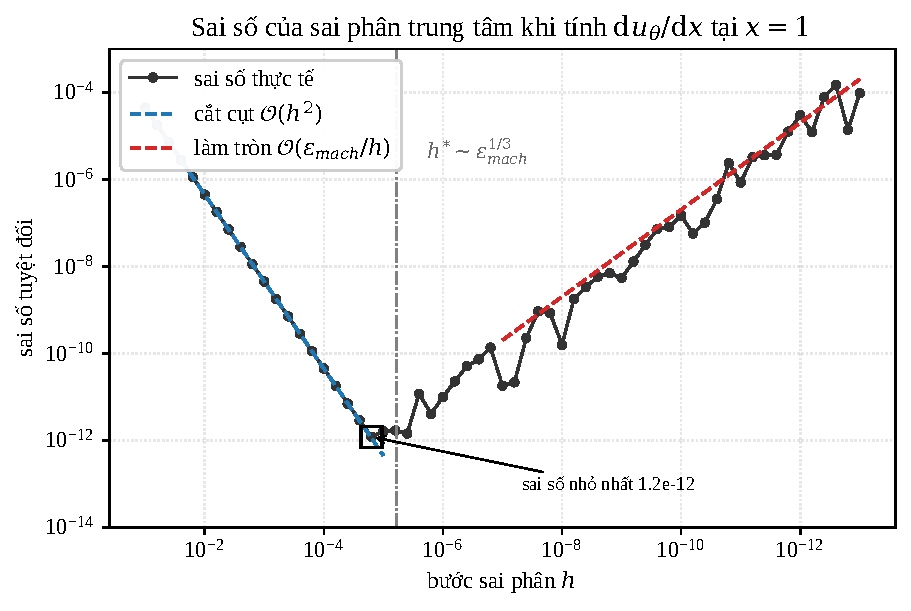
\includegraphics[width=0.82\textwidth]{Images/chap_3/hinh_saiphan.pdf}
\caption{Sai số tuyệt đối của sai phân trung tâm khi tính
$\mathrm{d}\Net_{\btheta}/\mathrm{d}x$ tại $x=1$, thang log--log, trục hoành
hướng về phía $h$ nhỏ dần. Đường gạch màu xanh là tiệm cận cắt cụt
$\mathcal{O}(h^2)$, đường gạch màu đỏ là tiệm cận làm tròn
$\mathcal{O}(\eps/h)$. Không có cách chọn $h$ nào đưa sai số xuống dưới đáy hình
chữ V; vi phân tự động cho giá trị chính xác tới độ chính xác máy.}
\label{fig:saiphan}
\end{figure}
 
\begin{nhanxet}[Hệ quả đối với bài toán phương trình vi phân]
\label{nx:fd-pde}
Bảng~\ref{tab:fd-error} mới chỉ là đạo hàm bậc nhất. Ba lý do khiến tình hình xấu
đi nhanh chóng trong bối cảnh của báo cáo.
 
Thứ nhất, với đạo hàm bậc hai, lược đồ trung tâm
$\big(f(x+h)-2f(x)+f(x-h)\big)/h^2$ có sai số cắt cụt $\mathcal{O}(h^2)$ nhưng
sai số làm tròn $\mathcal{O}(\eps|f|/h^2)$; lặp lại lập luận của
Mệnh đề~\ref{md:fd-rao-can} cho $h^{*} \sim \eps^{1/4}$ và sai số tốt nhất chỉ
còn cỡ $\eps^{1/2} \approx 10^{-8}$. Mỗi bậc đạo hàm làm mất thêm vài bậc độ
chính xác.
 
Thứ hai, với miền $n_0$ chiều, mỗi đạo hàm riêng cần thêm hai lần đánh giá mạng,
nên chi phí nhân lên tuyến tính theo $n_0$ -- trong khi vi phân tự động cho toàn
bộ gradient trong một lượt.
 
Thứ ba, và quan trọng nhất: phần dư $\mathcal{L}[\Net_{\btheta}] - f$ được đưa
\emph{trực tiếp} vào hàm mục tiêu rồi lại được lấy đạo hàm theo $\btheta$. Sai số
$10^{-8}$ ở phần dư không chỉ làm hàm mục tiêu sai lệch, nó còn tạo ra một
gradient sai lệch mà thuật toán tối ưu sẽ trung thành đi theo. Nói cách khác, sai
số xấp xỉ ở bước này không bị dập tắt mà được khuếch đại qua toàn bộ quá trình
huấn luyện, và nó đặt một sàn cứng lên độ chính xác cuối cùng của nghiệm. Đây là
lý do vì sao phương pháp PINN ở Chương~\ref{chap:pinn} bắt buộc dùng vi phân tự
động; Raissi và cộng sự~\cite{raissi2019} nêu điều này như một điều kiện của
phương pháp chứ không phải một lựa chọn cài đặt.
\end{nhanxet}
 
\subsection{Chế độ thuận}
\label{subsec:forward-mode}
 
Xét hàm $f : \R^n \to \R^m$ được tính bởi dãy phép toán sơ cấp $v_1,\dots,v_K$
theo đồ thị của Định nghĩa~\ref{def:comp-graph}. Cố định một \emph{vectơ mầm}
(seed) $\bm{r} \in \R^n$. \emph{Chế độ thuận} gắn kèm mỗi biến $v_k$ một
\emph{đạo hàm thuận} (tangent)
\begin{equation}
\dot{v}_k \coloneqq \frac{\partial v_k}{\partial \bx}\, \bm{r},
\label{eq:tangent}
\end{equation}
tức đạo hàm có hướng của $v_k$ theo hướng $\bm{r}$, rồi lan truyền $\dot{v}_k$
\emph{cùng chiều} với lượt tính giá trị, theo quy tắc dây chuyền
\begin{equation}
\dot{v}_k = \sum_{j \in \mathrm{Pa}(k)}
  \frac{\partial \varphi_k}{\partial v_j}\, \dot{v}_j ,
\qquad
\dot{\bx} = \bm{r}.
\label{eq:forward-truy-hoi}
\end{equation}
Kết thúc lượt, $\dot{\bm{y}} = \D f(\bx)\,\bm{r}$: một lượt chế độ thuận cho ta
\emph{tích Jacobi--vectơ} (Jacobian--vector product, JVP). Muốn có toàn bộ ma
trận Jacobi $m\times n$, cần $n$ lượt với $\bm{r} = \bm{e}_1,\dots,\bm{e}_n$. Vậy
chế độ thuận \emph{hiệu quả khi $n \ll m$}.
 
Cách phát biểu cô đọng nhất của \eqref{eq:forward-truy-hoi} là qua số đối ngẫu.
 
\begin{definition}[Số đối ngẫu]
\label{def:doi-ngau}
Vành số đối ngẫu là $\mathbb{D} = \{ a + b\epsilon : a,b \in \R \}$ với phép
cộng và nhân thông thường cùng quy tắc $\epsilon^2 = 0$, $\epsilon \neq 0$.
\end{definition}
 
\begin{bode}[Nguyên lý của chế độ thuận]
\label{bd:doi-ngau}
Nếu $f$ khả vi tại $a$ thì, trong $\mathbb{D}$,
\begin{equation}
f(a + b\epsilon) = f(a) + f'(a)\, b\, \epsilon .
\label{eq:doi-ngau}
\end{equation}
\end{bode}
 
\begin{proof}
Với $f$ đa thức, khai triển $(a+b\epsilon)^k = a^k + k a^{k-1}b\epsilon$ theo
nhị thức Newton: mọi số hạng chứa $\epsilon^2$ trở lên đều triệt tiêu do
$\epsilon^2 = 0$. Lấy tổ hợp tuyến tính cho \eqref{eq:doi-ngau} với $f$ đa thức.
Với $f$ tổng quát khả vi, \eqref{eq:doi-ngau} được \emph{lấy làm định nghĩa} của
phép mở rộng $f$ lên $\mathbb{D}$; định nghĩa này nhất quán với phép hợp thành,
vì
\[
(g\circ f)(a+b\epsilon) = g\big(f(a) + f'(a)b\,\epsilon\big)
 = g(f(a)) + g'(f(a))f'(a)\,b\,\epsilon,
\]
đúng bằng quy tắc dây chuyền.
\end{proof}
 
Bổ đề~\ref{bd:doi-ngau} cho một cài đặt ngắn gọn đến bất ngờ: chỉ cần \emph{nạp
chồng} các phép toán số học cho kiểu số đối ngẫu rồi đánh giá $f$ tại
$x + 1\cdot\epsilon$; phần $\epsilon$ của kết quả chính là $f'(x)$, chính xác,
không cần chọn $h$. Toàn bộ vấn đề của Mệnh đề~\ref{md:fd-rao-can} biến mất, vì
ở đây không có phép trừ hai số gần nhau nào cả.
 
\subsection{Chế độ ngược}
\label{subsec:reverse-mode}
 
Đối ngẫu với chế độ thuận, \emph{chế độ ngược} cố định một vectơ mầm
$\bm{w} \in \R^m$ ở phía đầu ra và gắn kèm mỗi biến một \emph{biến liên hợp}
(adjoint)
\begin{equation}
\bar{v}_k \coloneqq \frac{\partial \big(\bm{w}^{\top} f\big)}{\partial v_k},
\label{eq:adjoint}
\end{equation}
rồi lan truyền chúng \emph{ngược chiều} đồ thị theo \eqref{eq:chain-graph}. Kết
thúc lượt, $\bar{\bx} = \bm{w}^{\top}\D f(\bx)$: một lượt cho ta tích
vectơ--Jacobi \eqref{eq:vjp}. Cần $m$ lượt để có toàn bộ Jacobi, nên chế độ ngược
\emph{hiệu quả khi $m \ll n$}.
 
\begin{nhanxet}
\label{nx:bp-is-reverse}
Lan truyền ngược ở Mục~\ref{sec:backprop} chính là chế độ ngược áp dụng cho
trường hợp $m = 1$ (hàm mục tiêu vô hướng, $\bm{w} = 1$) và $n = P$ (số tham
số). Đây là kịch bản cực đoan nhất về tỉ lệ $m/n$, và cũng là lý do khiến chế độ
ngược thống trị trong học sâu. Mối liên hệ này giải thích vì sao mọi thư viện
hiện đại~\cite{paszke2019} chỉ cài đặt một cơ chế vi phân tự động chung, còn
``lan truyền ngược'' chỉ là tên gọi lịch sử của một trường hợp riêng. Nó cũng
giải thích vì sao Mệnh đề~\ref{md:bp}, dù được chứng minh riêng cho mạng truyền
thẳng, không cần chứng minh lại khi ta thêm phần dư phương trình vi phân vào đồ
thị.
\end{nhanxet}
 
\begin{dinhly}[Nguyên lý gradient rẻ]
\label{dl:cheap-gradient}
Với mọi hàm $f:\R^n \to \R$ được tính bởi một chương trình gồm các phép toán sơ
cấp, chế độ ngược tính $\nabla f$ với số phép toán không vượt quá một hằng số
nhân với số phép toán đánh giá $f$, và hằng số ấy \emph{không phụ thuộc $n$}.
\end{dinhly}
 
Giá trị chính xác của hằng số phụ thuộc mô hình chi phí được dùng; các chặn
thường được trích dẫn nằm trong khoảng $3$ đến $5$~\cite{griewank2008}.
Mệnh đề~\ref{md:chi-phi-bp} là trường hợp riêng của
Định lý~\ref{dl:cheap-gradient} cho mạng truyền thẳng, ở đó ta tính được hằng số
cụ thể $c \le 3$ nhờ biết rõ cấu trúc đồ thị.
 
Đánh đổi là bộ nhớ: chế độ ngược phải lưu (hoặc tính lại) mọi giá trị trung gian
của lượt thuận, nên chi phí bộ nhớ tỉ lệ với \emph{độ dài} của đồ thị tính toán.
Điều này trở nên đáng kể khi ta lấy đạo hàm bậc cao ở mục sau.
 
\begin{table}[htbp]
\centering
\caption{So sánh hai chế độ vi phân tự động cho $f:\R^n\to\R^m$.}
\label{tab:ad-modes}
\begin{tabular}{@{}lll@{}}
\toprule
 & Chế độ thuận & Chế độ ngược \\
\midrule
Đại lượng lan truyền   & tangent $\dot{v}$          & adjoint $\bar{v}$ \\
Chiều lan truyền       & cùng chiều đồ thị          & ngược chiều đồ thị \\
Một lượt cho ta        & $\D f\,\bm{r}$ (JVP)       & $\bm{w}^{\top}\D f$ (VJP) \\
Số lượt cho Jacobi đầy & $n$                        & $m$ \\
Hiệu quả khi           & $n \ll m$                  & $m \ll n$ \\
Bộ nhớ                 & $\mathcal{O}(1)$ theo độ dài đồ thị
                       & $\mathcal{O}(\text{độ dài đồ thị})$ \\
\bottomrule
\end{tabular}
\end{table}
 
\subsection{Đạo hàm theo biến đầu vào và đạo hàm bậc cao}
\label{subsec:bac-cao-ad}
 
Đây là mục có ý nghĩa quyết định đối với phần còn lại của báo cáo, và là mắt
xích nối trở lại Chương~\ref{chap:fnn}. Khi giải phương trình vi phân, mạng
$\Net_{\btheta}(\bx)$ đóng vai trò hàm thử và ta cần các đại lượng
$\partial_{x_i}\Net_{\btheta}$, $\partial^2_{x_ix_j}\Net_{\btheta}$, sau đó lại
phải lấy đạo hàm của toàn bộ biểu thức ấy theo $\btheta$.
 
Điểm mấu chốt là: \emph{đầu ra của một lượt vi phân tự động cũng là một hàm được
tính bởi một đồ thị tính toán}. Do đó có thể áp dụng vi phân tự động lên chính
nó. Mệnh đề sau làm rõ rằng cơ chế này không phải một thủ thuật lập trình mà tái
tạo đúng các hệ thức truy hồi đã được chứng minh ở Chương~\ref{chap:fnn}.
 
\begin{menhde}[Vi phân tự động tái tạo các truy hồi \eqref{eq:G-truy-hoi} và
\eqref{eq:S-truy-hoi}]
\label{md:ad-tai-tao}
Xét mạng theo Định nghĩa~\ref{def:fnn} với $\sigma \in C^2$ và $n_L = 1$.
 
\emph{(a)} Một lượt chế độ thuận trên đồ thị của lượt xuôi, với vectơ mầm
$\dot{\bx} = \bm{r}$, sinh ra dãy tangent $\dot{\ba}^{(\ell)}$ thoả đúng
\begin{equation}
\dot{\ba}^{(\ell)} = \bD^{(\ell)}\bW^{(\ell)}\dot{\ba}^{(\ell-1)},
\qquad \dot{\ba}^{(0)} = \bm{r},
\label{eq:ad-jvp}
\end{equation}
tức $\dot{\ba}^{(\ell)} = \bG^{(\ell)}\bm{r}$ với $\bG^{(\ell)}$ của
Mệnh đề~\ref{md:jacobian}. Do đó $n_0$ lượt thuận với các mầm
$\bm{e}_1,\dots,\bm{e}_{n_0}$ cho đúng ma trận $\partial_{\bx}\Net_{\btheta}$
của \eqref{eq:jacobian}.
 
\emph{(b)} Một lượt chế độ thuận với mầm $\bm{r}$ áp lên đồ thị \emph{mở rộng}
đã chứa $\dot{\ba}^{(\ell)}$ (tức chế độ thuận trên chế độ thuận) sinh ra dãy
$\ddot{\ba}^{(\ell)}$ thoả
\begin{equation}
\ddot{a}^{(\ell)}_k
 = \sigma''\!\big(z^{(\ell)}_k\big)\big(\dot{z}^{(\ell)}_k\big)^2
 + \sigma'\!\big(z^{(\ell)}_k\big)
   \sum_{j} w^{(\ell)}_{kj}\,\ddot{a}^{(\ell-1)}_j,
\qquad \ddot{\ba}^{(0)} = \bm{0},
\label{eq:ad-hvp}
\end{equation}
tức $\ddot{a}^{(\ell)}_k = \bm{r}^{\top}\bS^{(\ell)}_k\bm{r}$ với
$\bS^{(\ell)}_k$ của Mệnh đề~\ref{md:hessian}. Nói riêng, mỗi lượt như vậy cho
\emph{một dạng toàn phương} $\bm{r}^{\top}\nabla^2_{\bx}\Net_{\btheta}\,\bm{r}$
của Hessian, và với $\bm{r} = \bm{e}_i$ ta được đúng
$\partial^2_{x_i x_i}\Net_{\btheta}$.
\end{menhde}
 
\begin{proof}
\emph{(a)} Áp dụng \eqref{eq:forward-truy-hoi} cho hai phép toán sơ cấp của lớp
$\ell$. Với phép affine \eqref{eq:fnn-affine}, các đỉnh cha của $\bz^{(\ell)}$ là
$\ba^{(\ell-1)}$ (cùng $\bW^{(\ell)},\bb^{(\ell)}$, vốn có tangent bằng $0$ vì
$\btheta$ không phụ thuộc $\bx$), và
$\partial\bz^{(\ell)}/\partial\ba^{(\ell-1)} = \bW^{(\ell)}$, cho
$\dot{\bz}^{(\ell)} = \bW^{(\ell)}\dot{\ba}^{(\ell-1)}$. Với phép kích hoạt
\eqref{eq:fnn-act}, Jacobi là $\bD^{(\ell)}$, cho
$\dot{\ba}^{(\ell)} = \bD^{(\ell)}\dot{\bz}^{(\ell)}$. Ghép hai bước được
\eqref{eq:ad-jvp}, trùng với \eqref{eq:G-truy-hoi} nhân phải với $\bm{r}$. Quy
nạp theo $\ell$ với cơ sở $\dot{\ba}^{(0)} = \bm{r} = \bG^{(0)}\bm{r}$ cho
$\dot{\ba}^{(\ell)} = \bG^{(\ell)}\bm{r}$.
 
\emph{(b)} Lấy đạo hàm có hướng theo $\bm{r}$ của hai hệ thức trong \emph{(a)}.
Với phép affine, $\ddot{\bz}^{(\ell)} = \bW^{(\ell)}\ddot{\ba}^{(\ell-1)}$, tức
$\ddot{z}^{(\ell)}_k = \sum_j w^{(\ell)}_{kj}\ddot{a}^{(\ell-1)}_j$. Với phép
kích hoạt, $\dot{a}^{(\ell)}_k = \sigma'(z^{(\ell)}_k)\dot{z}^{(\ell)}_k$ là
tích của hai đại lượng cùng phụ thuộc $\bx$, nên quy tắc tích cho
\[
\ddot{a}^{(\ell)}_k
 = \sigma''\!\big(z^{(\ell)}_k\big)\big(\dot z^{(\ell)}_k\big)^2
 + \sigma'\!\big(z^{(\ell)}_k\big)\,\ddot{z}^{(\ell)}_k ,
\]
đúng bằng \eqref{eq:ad-hvp}. Để nhận ra đây là dạng toàn phương của
$\bS^{(\ell)}_k$, nhân hai vế của \eqref{eq:S-truy-hoi} với $\bm{r}^{\top}$ bên
trái và $\bm{r}$ bên phải: số hạng thứ nhất cho
$\sigma''(z^{(\ell)}_k)\big(\bm{g}^{(\ell)}_k\bm{r}\big)^2$, và
$\bm{g}^{(\ell)}_k\bm{r} = \dot z^{(\ell)}_k$ theo \emph{(a)}; số hạng thứ hai
cho $\sigma'(z^{(\ell)}_k)\sum_j w^{(\ell)}_{kj}\,
\bm{r}^{\top}\bS^{(\ell-1)}_j\bm{r}$. Hai vế thoả cùng một truy hồi với cùng điều
kiện đầu ($\bS^{(0)}_k = \bm{0}$ và $\ddot{\ba}^{(0)} = \bm{0}$), nên trùng nhau
theo quy nạp.
\end{proof}
 
\begin{nhanxet}[Ý nghĩa của Mệnh đề~\ref{md:ad-tai-tao}]
Ba kết luận thực hành.
 
Thứ nhất, người dùng \emph{không phải lập trình} $\sigma''$: thư viện chỉ biết
đạo hàm của các phép toán sơ cấp và tự sinh ra số hạng $\sigma''(z_k)\dot z_k^2$
qua quy tắc tích. Đây là điểm khác biệt căn bản với
Thuật toán~\ref{alg:dao-ham}, vốn đòi hỏi viết tường minh công thức
\eqref{eq:tanh-d2}.
 
Thứ hai, mỗi lượt cho một dạng toàn phương chứ không phải toàn bộ Hessian. Muốn
đủ $\nabla^2_{\bx}\Net_{\btheta}$ cần $\mathcal{O}(n_0)$ lượt (hoặc
$\mathcal{O}(n_0^2)$ nếu lấy từng phần tử riêng lẻ), khớp với ước lượng chi phí ở
Nhận xét~\ref{nx:chi-phi-hessian}. Với phương trình Laplace hay khuếch tán, thứ
cần thiết là \emph{vết} $\sum_i \partial^2_{x_ix_i}\Net_{\btheta}$, tức $n_0$
lượt với các mầm $\bm{e}_i$ -- không cần Hessian đầy đủ.
 
Thứ ba, đây là kết quả về \emph{tính đúng đắn}, không phải về chiến lược cài đặt
tối ưu. Trong PyTorch, cách thông dụng là dùng chế độ ngược hai lần thay vì chế
độ thuận hai lần; hai cách cho cùng kết quả nhưng khác nhau về chi phí bộ nhớ.
\end{nhanxet}
 
\paragraph{Ba lượt của một bước huấn luyện PINN.}
Với phương trình $u_t = \nu u_{xx}$, một bước huấn luyện gồm:
\begin{enumerate}[label=(\arabic*), leftmargin=*]
\item Lượt thứ nhất (chế độ ngược, \emph{giữ lại} đồ thị) cho $\partial_x
      \Net_{\btheta}$ và $\partial_t\Net_{\btheta}$ như những đỉnh mới trong đồ
      thị mở rộng.
\item Lượt thứ hai áp lên $\partial_x\Net_{\btheta}$ cho
      $\partial^2_{xx}\Net_{\btheta}$, từ đó dựng phần dư
      $\mathcal{R} = \partial_t\Net_{\btheta} - \nu\,\partial^2_{xx}
      \Net_{\btheta}$ và hàm mục tiêu $J$.
\item Lượt thứ ba lấy $\nabla_{\btheta} J$ trên toàn bộ đồ thị mở rộng, phục vụ
      bước cập nhật tối ưu.
\end{enumerate}
Trong PyTorch~\cite{paszke2019}, hai lượt đầu tương ứng với việc gọi
\texttt{torch.autograd.grad(u, x, create\_graph=True)}, trong đó cờ
\texttt{create\_graph} báo cho hệ thống rằng bản thân phép tính gradient phải được
\emph{ghi lại} vào băng ghi thay vì bị loại bỏ sau khi dùng. Bỏ sót cờ này là lỗi
cài đặt phổ biến nhất khi triển khai PINN: chương trình vẫn chạy, hàm mục tiêu
vẫn được tính, nhưng $\nabla_{\btheta} J$ bỏ mất toàn bộ đóng góp đi qua phần dư,
và mạng học ra một hàm không liên quan đến phương trình.
 
\begin{nhanxet}[Chi phí của đạo hàm bậc cao]
\label{nx:chi-phi-bac-cao}
Mỗi bậc đạo hàm nhân độ dài đồ thị lên một hằng số. Với phương trình bậc hai như
phương trình khuếch tán hay Burgers, đồ thị dùng cho lượt tối ưu hoá dài gấp
khoảng bốn đến sáu lần đồ thị của lượt xuôi thuần tuý, và bộ nhớ tăng theo cùng
tỉ lệ do Định lý~\ref{dl:cheap-gradient} đòi hỏi lưu toàn bộ giá trị trung gian.
Ước lượng ``bốn đến sáu'' ở đây là ước lượng \emph{a priori}, và phép đo ở
Mục~\ref{sec:tn9} cho thấy nó \emph{thấp}: bội số đo được là khoảng chín. Sai
lệch nằm ở chỗ ước lượng này ngầm coi hai bậc đạo hàm tốn như nhau, trong khi
lượt lấy $\partial_{xx}u$ chạy ngược trên đồ thị đã được lượt lấy
$\partial_{x}u$ nối dài; xem phần thảo luận ở Mục~\ref{sec:tn9}.
Đây là nguyên nhân chính khiến một bước huấn luyện PINN đắt hơn đáng kể so với
một bước huấn luyện mạng hồi quy cùng kích thước, và là lý do phải chọn hàm kích
hoạt trơn: với ReLU, $\sigma'' \equiv 0$ hầu khắp nơi
(Hệ quả~\ref{hq:relu-hkn}), số hạng thứ nhất của \eqref{eq:ad-hvp} triệt tiêu ở
mọi lớp, và theo Hệ quả~\ref{hq:pinn-hong} hàm mục tiêu trở thành hằng số địa
phương.
\end{nhanxet}
 
\begin{nhanxet}[Kết hợp hai chế độ]
Khi cần tích Hessian--vectơ $\nabla^2_{\btheta} J(\btheta)\,\bm{r}$ -- đại lượng
xuất hiện trong các phương pháp Newton chặt cụt -- cách hiệu quả nhất là
\emph{thuận trên ngược}: áp dụng chế độ thuận lên đồ thị của lượt ngược. Lý do
nằm ở Bảng~\ref{tab:ad-modes}: lượt ngược cho hàm
$\btheta \mapsto \nabla_{\btheta}J \in \R^P$, và ta chỉ cần JVP của hàm này theo
một hướng, tức đúng việc mà chế độ thuận làm trong một lượt. Chi phí do đó chỉ
tương đương một vài lần đánh giá $J$, thay vì $\mathcal{O}(P^2)$ nếu dựng tường
minh Hessian.
\end{nhanxet}
 
%==============================================================================
\section{Các thuật toán tối ưu}
\label{sec:optimizers}
%==============================================================================
 
\subsection{Đặc thù của bài toán}
\label{subsec:dac-thu}
 
Bài toán \eqref{eq:erm} có ba đặc điểm quy định việc lựa chọn thuật toán, và cả
ba đều đã được thiết lập ở các chương trước chứ không phải giả định.
 
\emph{Không lồi.} Mệnh đề~\ref{md:khong-loi} cho thấy $J$ không lồi do đối xứng
dấu, và Nhận xét~\ref{nx:doi-xung-hoan-vi} cho thấy mỗi cực tiểu sinh ra ít nhất
$2^{n_1}n_1!$ cực tiểu tương đương. Ta chỉ có thể kỳ vọng tìm được \emph{điểm
dừng}, không phải cực tiểu toàn cục.
 
\emph{Chiều rất lớn.} $P$ cho bởi \eqref{eq:so-tham-so} thường ở mức $10^3$ đến
$10^7$, nên mọi phương pháp cần lưu ma trận $P\times P$ đều bị loại ngay.
 
\emph{Điều kiện xấu.} Trong bối cảnh phương trình vi phân, hàm mục tiêu
\eqref{eq:pinn-loss} tổ hợp nhiều thành phần có thứ nguyên và thang độ khác nhau
-- phần dư phương trình, điều kiện biên, điều kiện ban đầu -- tạo ra một Hessian
có số điều kiện lớn.
 
Mọi thuật toán dưới đây đều thuộc lược đồ lặp chung
\begin{equation}
\btheta_{k+1} = \btheta_k + \alpha_k \bm{p}_k,
\label{eq:iter-scheme}
\end{equation}
và chỉ khác nhau ở cách chọn \emph{hướng} $\bm{p}_k$ và \emph{độ dài bước}
$\alpha_k$~\cite{nocedal2006}.
 
\subsection{Hạ gradient và hạ gradient ngẫu nhiên}
\label{subsec:sgd}
 
Lựa chọn đơn giản nhất là $\bm{p}_k = -\nabla J(\btheta_k)$, hướng giảm nhanh
nhất tại chỗ. Với $N$ lớn, việc tính đủ tổng trong \eqref{eq:erm} ở mỗi bước quá
tốn kém, nên ta thay bằng ước lượng không chệch trên một lô nhỏ
$\mathcal{B}_k \subset \{1,\dots,N\}$:
\begin{equation}
\bm{g}_k = \frac{1}{|\mathcal{B}_k|}\sum_{i \in \mathcal{B}_k}
\nabla_{\btheta}\, \varrho\!\left(\Net_{\btheta_k}(\bx_i), \bm{y}_i\right),
\qquad
\btheta_{k+1} = \btheta_k - \alpha_k \bm{g}_k .
\label{eq:sgd}
\end{equation}
Trình bày về hạ gradient ngẫu nhiên và các biến thể của nó ở mục này theo
Goodfellow và cộng sự~\cite{goodfellow2016}.
 
\begin{dinhly}[Hội tụ dưới điều kiện bước học Robbins--Monro]
\label{dl:robbins-monro}
Giả sử $J$ khả vi liên tục, bị chặn dưới, $\nabla J$ Lipschitz, ước lượng
$\bm{g}_k$ không chệch và có phương sai bị chặn. Nếu dãy bước học thoả mãn
\begin{equation}
\sum_{k=1}^{\infty} \alpha_k = \infty,
\qquad
\sum_{k=1}^{\infty} \alpha_k^2 < \infty,
\label{eq:rm}
\end{equation}
thì $J(\btheta_k)$ hội tụ hầu chắc chắn và
$\liminf_{k\to\infty}\|\nabla J(\btheta_k)\| = 0$ hầu chắc chắn.
\end{dinhly}
 
Hai điều kiện trong \eqref{eq:rm} có ý nghĩa đối lập và đều cần thiết. Điều kiện
thứ nhất bảo đảm thuật toán có thể đi được quãng đường tuỳ ý -- nếu
$\sum\alpha_k < \infty$ thì $\btheta_k$ bị nhốt trong một hình cầu quanh
$\btheta_0$ và không thể tới nghiệm nếu nghiệm nằm ngoài. Điều kiện thứ hai bảo
đảm nhiễu ngẫu nhiên bị dập tắt dần. Cặp điều kiện này xuất phát từ Robbins và
Monro trong bài toán tìm nghiệm ngẫu nhiên; phát biểu cho trường hợp không lồi
như trên thuộc về Bertsekas và Tsitsiklis~\cite{bertsekas2000}.
 
Trong thực hành, người ta hiếm khi dùng dãy $\alpha_k$ thoả \eqref{eq:rm} một
cách nghiêm ngặt, mà dùng bước học hằng số theo từng giai đoạn rồi giảm dần theo
lịch. Mệnh đề sau lượng hoá cái giá phải trả cho sự thoả hiệp đó.
 
\begin{menhde}[Sàn nhiễu của bước học hằng số]
\label{md:san-nhieu}
Xét mô hình bậc hai một chiều $J(\theta) = \tfrac{\mu}{2}\theta^2$ với $\mu > 0$,
và bước lặp \eqref{eq:sgd} với bước học hằng số $\alpha \in (0, 2/\mu)$ và
gradient nhiễu $g_k = \mu\theta_k + \xi_k$, trong đó $\xi_k$ độc lập, kỳ vọng
$0$, phương sai $\varsigma^2$. Khi đó
\begin{equation}
\lim_{k\to\infty}\E\big[\theta_k^2\big]
 = \frac{\alpha\,\varsigma^{2}}{\mu\,(2-\alpha\mu)},
\qquad
\lim_{k\to\infty}\E\big[J(\theta_k)\big]
 = \frac{\alpha\,\varsigma^{2}}{2\,(2-\alpha\mu)},
\label{eq:san-nhieu}
\end{equation}
và do đó $\lim_{k\to\infty}\E[J(\theta_k)] \sim \alpha\varsigma^{2}/4$ khi
$\alpha \to 0^{+}$.
\end{menhde}
 
\begin{proof}
Thay $g_k$ vào \eqref{eq:sgd}:
$\theta_{k+1} = (1-\alpha\mu)\theta_k - \alpha\xi_k$. Đặt
$s_k = \E[\theta_k^2]$. Vì $\xi_k$ độc lập với $\theta_k$ và có kỳ vọng $0$, số
hạng chéo triệt tiêu khi bình phương và lấy kỳ vọng:
\[
s_{k+1} = (1-\alpha\mu)^2 s_k + \alpha^2\varsigma^2 .
\]
Đây là truy hồi affine với hệ số $q := (1-\alpha\mu)^2 \in [0,1)$ khi
$\alpha \in (0,2/\mu)$, nên $s_k$ hội tụ tới điểm bất động
$s_\infty = \alpha^2\varsigma^2/(1-q)$. Khai triển
$1 - q = 2\alpha\mu - \alpha^2\mu^2 = \alpha\mu(2-\alpha\mu)$ cho
\eqref{eq:san-nhieu}. Đẳng thức thứ hai theo $J = \tfrac{\mu}{2}\theta^2$.
\end{proof}
 
\begin{nhanxet}[Sàn nhiễu]
\label{nx:noise-floor}
Mệnh đề~\ref{md:san-nhieu} cho một kết luận sắc nét: với bước học hằng số, dãy
$\btheta_k$ \emph{không} hội tụ tới điểm dừng mà chỉ dao động trong một lân cận,
và giá trị kỳ vọng của hàm mục tiêu bị chặn dưới bởi một mức tỉ lệ \emph{tuyến
tính} với $\alpha$ và với phương sai của gradient. Muốn giảm sàn nhiễu mười lần,
phải giảm bước học mười lần, và khi ấy tốc độ tiến tới lân cận cũng chậm đi
tương ứng -- hệ số co là $(1-\alpha\mu)$.
 
Hiện tượng này là giới hạn cơ bản của mọi phương pháp ngẫu nhiên bậc nhất, không
phải một khiếm khuyết cài đặt, và nó là lập luận trung tâm ở
Mục~\ref{subsec:adam-vs-lbfgs}. Cần nói rõ phạm vi: mệnh đề được chứng minh cho
mô hình bậc hai một chiều, tức là một mô hình địa phương quanh điểm cực tiểu, chứ
không phải cho hàm mục tiêu PINN đầy đủ. Nó giải thích hiện tượng chững lại quan
sát được ở Hình~\ref{fig:hoitu}, nhưng không phải là một định lý về hàm mục tiêu
ấy.
\end{nhanxet}
 
\subsection{Động lượng}
\label{subsec:momentum}
 
Hạ gradient thuần tuý tiến rất chậm trong các ``khe hẹp'' của hàm mục tiêu: nó
dao động qua lại theo hướng có độ cong lớn và bò rất chậm theo hướng có độ cong
nhỏ. Phương pháp \emph{động lượng}~\cite{goodfellow2016} khắc phục bằng cách tích
luỹ một trung bình trượt của các gradient quá khứ:
\begin{equation}
\bm{v}_k = \beta \bm{v}_{k-1} - \alpha \bm{g}_k,
\qquad
\btheta_{k+1} = \btheta_k + \bm{v}_k,
\qquad \beta \in [0,1).
\label{eq:momentum}
\end{equation}
 
\begin{bode}[Hệ số khuếch đại của động lượng]
\label{bd:momentum}
Giả sử $\bm{g}_k \equiv \bm{g}$ không đổi và $\bm{v}_0 = \bm{0}$. Khi đó
\begin{equation}
\bm{v}_k = -\alpha\,\frac{1-\beta^{k}}{1-\beta}\,\bm{g}
\;\xrightarrow[k\to\infty]{}\;
-\frac{\alpha}{1-\beta}\,\bm{g}.
\label{eq:momentum-khuech-dai}
\end{equation}
Ngược lại, nếu $\bm{g}_k$ đổi dấu luân phiên, $\bm{g}_k = (-1)^k\bm{g}$, thì
\begin{equation}
\bm{v}_k = -\alpha\,(-1)^{k}\,\frac{1-(-\beta)^{k}}{1+\beta}\,\bm{g},
\qquad\text{nên}\qquad
\norm{\bm{v}_k} \;\xrightarrow[k\to\infty]{}\;
  \frac{\alpha\,\norm{\bm{g}}}{1+\beta},
\label{eq:momentum-dao-dong}
\end{equation}
tức biên độ bị \emph{thu nhỏ} đi thừa số $1/(1+\beta)$ (bản thân $\bm{v}_k$ không
hội tụ, nó dao động đổi dấu theo $k$).
\end{bode}
 
\begin{proof}
Khai triển truy hồi \eqref{eq:momentum}:
$\bm{v}_k = -\alpha\sum_{j=0}^{k-1}\beta^{j}\bm{g}_{k-j}$. Với $\bm{g}_k \equiv
\bm{g}$, tổng là cấp số nhân $\sum_{j=0}^{k-1}\beta^j = (1-\beta^k)/(1-\beta)$,
cho \eqref{eq:momentum-khuech-dai}. Với $\bm{g}_{k-j} = (-1)^{k-j}\bm{g}
= (-1)^{k}(-1)^{j}\bm{g}$, tổng trở thành
$(-1)^k\sum_{j=0}^{k-1}(-\beta)^{j} = (-1)^k\,\dfrac{1-(-\beta)^{k}}{1+\beta}$,
cho \eqref{eq:momentum-dao-dong}; vì $|\beta| < 1$ nên $(-\beta)^k \to 0$ và
chuẩn của $\bm{v}_k$ hội tụ tới $\alpha\norm{\bm{g}}/(1+\beta)$.
\end{proof}
 
Bổ đề~\ref{bd:momentum} giải thích chính xác cơ chế của động lượng: thành phần
\emph{nhất quán} của gradient được khuếch đại lên $1/(1-\beta)$ lần, còn thành
phần \emph{dao động} bị nén xuống $1/(1+\beta)$ lần. Với $\beta = 0{,}9$, tỉ số
giữa hai hệ số là $(1+\beta)/(1-\beta) = 19$: động lượng làm tăng độ tương phản
giữa hướng có ích và hướng dao động lên gần hai mươi lần. Biến thể
\emph{Nesterov} đánh giá gradient tại điểm đã được đẩy tới trước,
$\btheta_k + \beta\bm{v}_{k-1}$, tạo hiệu ứng ``nhìn trước'' giúp giảm vọt lố khi
tới gần điểm cực tiểu.
 
\subsection{Phương pháp thích nghi và thuật toán Adam}
\label{subsec:adam}
 
Ý tưởng tiếp theo là dùng bước học \emph{riêng cho từng toạ độ}, tự động thu nhỏ
ở những hướng có gradient lớn kéo dài. AdaGrad tích luỹ toàn bộ lịch sử bình
phương gradient, nên bước học giảm đơn điệu và có thể tắt quá sớm; RMSProp thay
tổng tích luỹ bằng trung bình trượt hàm mũ, khắc phục nhược điểm
đó~\cite{goodfellow2016}. Adam kết hợp
RMSProp với động lượng, đồng thời hiệu chỉnh độ chệch của các trung bình trượt ở
những bước đầu~\cite{kingma2015}.
 
\begin{algorithm}[htbp]
\caption{Adam}
\label{alg:adam}
\begin{algorithmic}[1]
\Require Bước học $\alpha$, hệ số $\beta_1,\beta_2 \in [0,1)$, hằng số
  $\varepsilon > 0$, tham số ban đầu $\btheta_0$
\State $\bm{m}_0 \gets \bm{0}$, \quad $\bm{v}_0 \gets \bm{0}$, \quad $k \gets 0$
\While{chưa thoả tiêu chuẩn dừng}
  \State $k \gets k+1$
  \State $\bm{g}_k \gets \nabla_{\btheta} J_{\mathcal{B}_k}(\btheta_{k-1})$
  \State $\bm{m}_k \gets \beta_1 \bm{m}_{k-1} + (1-\beta_1)\bm{g}_k$
    \Comment{mô-men bậc nhất}
  \State $\bm{v}_k \gets \beta_2 \bm{v}_{k-1}
    + (1-\beta_2)\, \bm{g}_k \odot \bm{g}_k$
    \Comment{mô-men bậc hai}
  \State $\hat{\bm{m}}_k \gets \bm{m}_k / (1-\beta_1^{\,k})$
    \Comment{hiệu chỉnh độ chệch, Bổ đề~\ref{bd:adam-bias}}
  \State $\hat{\bm{v}}_k \gets \bm{v}_k / (1-\beta_2^{\,k})$
  \State $\btheta_k \gets \btheta_{k-1} - \alpha\, \hat{\bm{m}}_k \big/
    \left(\sqrt{\hat{\bm{v}}_k} + \varepsilon\right)$
\EndWhile
\State \Return $\btheta_k$
\end{algorithmic}
\end{algorithm}
 
\begin{bode}[Vì sao cần hiệu chỉnh độ chệch]
\label{bd:adam-bias}
Giả sử $\bm{g}_1,\dots,\bm{g}_k$ cùng phân phối với $\E[\bm{g}_j] = \bm{g}$. Với
$\bm{m}_0 = \bm{0}$ và truy hồi ở dòng 5 của Thuật toán~\ref{alg:adam},
\begin{equation}
\E[\bm{m}_k] = \left(1-\beta_1^{\,k}\right)\bm{g},
\label{eq:adam-bias}
\end{equation}
nên $\bm{m}_k$ là ước lượng \emph{chệch} của $\bm{g}$, và
$\hat{\bm{m}}_k = \bm{m}_k/(1-\beta_1^k)$ là ước lượng không chệch. Kết luận
tương tự cho $\bm{v}_k$ với $\beta_2$.
\end{bode}
 
\begin{proof}
Khai triển truy hồi:
$\bm{m}_k = (1-\beta_1)\sum_{j=1}^{k}\beta_1^{\,k-j}\bm{g}_j$. Lấy kỳ vọng và
dùng tổng cấp số nhân:
$\E[\bm{m}_k] = (1-\beta_1)\,\bm{g}\sum_{j=1}^{k}\beta_1^{\,k-j}
= (1-\beta_1)\,\bm{g}\,\frac{1-\beta_1^{\,k}}{1-\beta_1}$, cho
\eqref{eq:adam-bias}.
\end{proof}
 
Bổ đề~\ref{bd:adam-bias} cho thấy độ chệch chỉ đáng kể ở những bước đầu: với
$\beta_1 = 0{,}9$, thừa số $1-\beta_1^k$ bằng $0{,}1$ tại $k=1$ nhưng đã vượt
$0{,}99$ tại $k = 44$. Với $\beta_2 = 0{,}999$, thời gian ``khởi động'' dài hơn
nhiều: cần $k \approx 4600$ để đạt cùng mức. Không hiệu chỉnh, các bước đầu tiên
sẽ có $\hat{\bm v}$ quá nhỏ và bước cập nhật quá lớn -- đúng lúc mô hình còn chưa
ổn định.
 
Giá trị mặc định được dùng phổ biến là $\alpha = 10^{-3}$, $\beta_1 = 0{,}9$,
$\beta_2 = 0{,}999$, $\varepsilon = 10^{-8}$; mọi phép toán ở dòng 5--9 đều thực
hiện theo từng thành phần.
 
\begin{nhanxet}[Bản chất của mẫu số trong Adam]
\label{nx:adam-duong-cheo}
Cần hiểu đúng bản chất của Adam: mẫu số $\sqrt{\hat{\bm{v}}_k}$ là một xấp xỉ
\emph{đường chéo} của thông tin bậc hai, ước lượng từ bình phương gradient chứ
không phải từ đạo hàm bậc hai thực sự. Nó chuẩn hoá thang độ giữa các toạ độ
nhưng \emph{không} nắm bắt được tương quan giữa chúng: nếu Hessian có dạng
$\begin{psmallmatrix} 1 & \gamma \\ \gamma & 1\end{psmallmatrix}$ với
$|\gamma|$ gần $1$, mọi xấp xỉ đường chéo đều thấy một ma trận đơn vị và bỏ sót
hoàn toàn số điều kiện $(1+\gamma)/(1-\gamma)$. Khi các hướng riêng của Hessian
nghiêng chéo so với hệ trục toạ độ -- điều xảy ra thường xuyên với hàm mục tiêu
của PINN, nơi các thành phần mất mát ràng buộc lẫn nhau qua cùng bộ trọng số --
xấp xỉ đường chéo không đủ. Đó chính là chỗ để phương pháp tựa Newton phát huy
tác dụng.
\end{nhanxet}
 
\subsection{Phương pháp tựa Newton và L-BFGS}
\label{subsec:lbfgs}
 
Xuất phát từ mô hình bậc hai của $J$ quanh $\btheta_k$,
\[
J(\btheta_k + \bm{p}) \approx J(\btheta_k)
 + \nabla J(\btheta_k)^{\top}\bm{p}
 + \tfrac{1}{2}\bm{p}^{\top}\nabla^2 J(\btheta_k)\,\bm{p},
\]
bước Newton là
$\bm{p}_k = -\big[\nabla^2 J(\btheta_k)\big]^{-1}\nabla J(\btheta_k)$. Bước này
hội tụ bậc hai ở lân cận nghiệm nhưng đòi hỏi dựng và nghịch đảo ma trận
$P\times P$ -- bất khả thi theo Mục~\ref{subsec:dac-thu}.
 
Các phương pháp \emph{tựa Newton} thay $\big[\nabla^2 J\big]^{-1}$ bằng một xấp
xỉ $\bm{H}_k$ được cập nhật từ chính các gradient đã tính. Đặt
\begin{equation}
\bm{s}_k = \btheta_{k+1}-\btheta_k,
\qquad
\bm{y}_k = \nabla J(\btheta_{k+1}) - \nabla J(\btheta_k).
\label{eq:s-y}
\end{equation}
Yêu cầu tự nhiên là $\bm{H}_{k+1}$ tái tạo đúng độ cong đã quan sát dọc
$\bm{s}_k$.
 
\begin{definition}[Phương trình cát tuyến]
\label{def:secant}
$\bm{H}_{k+1}\bm{y}_k = \bm{s}_k$.
\end{definition}
 
Phương trình cát tuyến là dạng nhiều chiều của phép xấp xỉ đạo hàm bậc hai bằng
sai phân của đạo hàm bậc nhất; nó có vô số nghiệm khi $P > 1$. Trong họ nghiệm
ấy, công thức BFGS chọn $\bm{H}_{k+1}$ gần $\bm{H}_k$ nhất theo một chuẩn có
trọng, đồng thời giữ tính đối xứng xác định dương:
\begin{equation}
\bm{H}_{k+1} = \left(\bm{I}-\rho_k \bm{s}_k \bm{y}_k^{\top}\right)
\bm{H}_k
\left(\bm{I}-\rho_k \bm{y}_k \bm{s}_k^{\top}\right)
+ \rho_k \bm{s}_k\bm{s}_k^{\top},
\qquad
\rho_k = \frac{1}{\bm{y}_k^{\top}\bm{s}_k}.
\label{eq:bfgs}
\end{equation}
Tính xác định dương được bảo toàn khi và chỉ khi thoả \emph{điều kiện độ cong}
$\bm{y}_k^{\top}\bm{s}_k > 0$. Điều kiện này không tự nhiên đúng, nhưng được bảo
đảm nếu độ dài bước $\alpha_k$ thoả các \emph{điều kiện Wolfe}
\begin{align}
J(\btheta_k + \alpha_k \bm{p}_k)
  &\le J(\btheta_k) + c_1 \alpha_k \nabla J(\btheta_k)^{\top}\bm{p}_k,
\label{eq:wolfe1}\\
\nabla J(\btheta_k + \alpha_k \bm{p}_k)^{\top}\bm{p}_k
  &\ge c_2\, \nabla J(\btheta_k)^{\top}\bm{p}_k,
\label{eq:wolfe2}
\end{align}
với $0 < c_1 < c_2 < 1$; thông dụng là $c_1 = 10^{-4}$, $c_2 = 0{,}9$.
 
\begin{bode}[Wolfe kéo theo điều kiện độ cong]
\label{bd:wolfe-curvature}
Nếu $\bm{p}_k$ là hướng giảm, tức $\nabla J(\btheta_k)^{\top}\bm{p}_k < 0$, và
$\alpha_k > 0$ thoả \eqref{eq:wolfe2}, thì
$\bm{y}_k^{\top}\bm{s}_k > 0$.
\end{bode}
 
\begin{proof}
Theo \eqref{eq:s-y} và \eqref{eq:iter-scheme}, $\bm{s}_k = \alpha_k\bm{p}_k$, nên
\[
\bm{y}_k^{\top}\bm{s}_k
 = \alpha_k\Big(\nabla J(\btheta_{k+1})^{\top}\bm{p}_k
   - \nabla J(\btheta_k)^{\top}\bm{p}_k\Big)
 \ge \alpha_k\,(c_2 - 1)\,\nabla J(\btheta_k)^{\top}\bm{p}_k,
\]
trong đó bất đẳng thức dùng \eqref{eq:wolfe2}. Vì $\alpha_k > 0$, $c_2 - 1 < 0$
và $\nabla J(\btheta_k)^{\top}\bm{p}_k < 0$, tích của ba thừa số là dương.
\end{proof}
 
Bổ đề~\ref{bd:wolfe-curvature} là lý do vì sao tìm kiếm đường Wolfe không phải
một chi tiết kỹ thuật có thể bỏ qua trong L-BFGS: bỏ nó đi thì $\bm{H}_k$ có thể
mất tính xác định dương, và khi ấy $\bm{p}_k$ không còn là hướng giảm.
 
Công thức \eqref{eq:bfgs} vẫn cần lưu ma trận đầy $P\times P$. Ý tưởng của
\emph{L-BFGS} (BFGS bộ nhớ hạn chế~\cite{liu1989}) là: không bao giờ dựng
$\bm{H}_k$, chỉ lưu $m$ cặp gần nhất
$\{(\bm{s}_i,\bm{y}_i)\}_{i=k-m}^{k-1}$ (thường $m$ từ $5$ đến $20$) và tính
\emph{tích} $\bm{H}_k\nabla J(\btheta_k)$ bằng một đệ quy hai vòng.
 
\begin{algorithm}[htbp]
\caption{Đệ quy hai vòng của L-BFGS}
\label{alg:two-loop}
\begin{algorithmic}[1]
\Require Gradient $\bm{g} = \nabla J(\btheta_k)$; các cặp
  $\{(\bm{s}_i,\bm{y}_i)\}_{i=k-m}^{k-1}$ với
  $\rho_i = 1/(\bm{y}_i^{\top}\bm{s}_i)$
\Ensure Hướng $\bm{p}_k = -\bm{H}_k \bm{g}$
\State $\bm{q} \gets \bm{g}$
\For{$i = k-1$ \textbf{xuống} $k-m$}
  \State $\alpha_i \gets \rho_i\, \bm{s}_i^{\top}\bm{q}$
  \State $\bm{q} \gets \bm{q} - \alpha_i \bm{y}_i$
\EndFor
\State $\gamma_k \gets \dfrac{\bm{s}_{k-1}^{\top}\bm{y}_{k-1}}
  {\bm{y}_{k-1}^{\top}\bm{y}_{k-1}}$
  \Comment{co giãn ma trận khởi tạo}
\State $\bm{r} \gets \gamma_k\, \bm{q}$
  \Comment{tức $\bm{H}_k^{0} = \gamma_k \bm{I}$}
\For{$i = k-m$ \textbf{đến} $k-1$}
  \State $\beta \gets \rho_i\, \bm{y}_i^{\top}\bm{r}$
  \State $\bm{r} \gets \bm{r} + \bm{s}_i\left(\alpha_i - \beta\right)$
\EndFor
\State \Return $\bm{p}_k = -\bm{r}$
\end{algorithmic}
\end{algorithm}
 
\begin{menhde}[Chi phí của đệ quy hai vòng]
\label{md:two-loop-cost}
Thuật toán~\ref{alg:two-loop} cần $\mathcal{O}(mP)$ phép toán số thực và
$\mathcal{O}(mP)$ ô nhớ, tuyến tính theo số tham số $P$.
\end{menhde}
 
\begin{proof}
Mỗi vòng lặp thực hiện đúng một tích vô hướng ($2P$ phép) và một phép cộng vectơ
có hệ số ($2P$ phép) trên các vectơ độ dài $P$; có $2m$ vòng lặp cả thảy, cộng
thêm phép co giãn ở dòng 5--6 tốn $\mathcal{O}(P)$. Bộ nhớ gồm $2m$ vectơ độ dài
$P$ cùng ba vectơ làm việc.
\end{proof}
 
Với $m = 10$ và $P = 10^4$, chi phí này không đáng kể so với một lượt lan truyền
ngược. Điểm mấu chốt là ma trận $\bm{H}_k$ -- vốn \emph{đầy} và chứa thông tin
tương quan giữa các toạ độ mà Nhận xét~\ref{nx:adam-duong-cheo} chỉ ra Adam
không có -- không bao giờ được dựng ra.
 
\begin{nhanxet}[Vì sao co giãn $\gamma_k$ lại quan trọng]
Ma trận khởi tạo $\bm{H}_k^{0} = \gamma_k \bm{I}$ với
$\gamma_k = \bm{s}_{k-1}^{\top}\bm{y}_{k-1} /
\bm{y}_{k-1}^{\top}\bm{y}_{k-1}$ là một ước lượng nghịch đảo của độ cong trung
bình theo hướng vừa đi qua: nếu $J$ là hàm bậc hai với Hessian $\bm{A}$ thì
$\bm{y} = \bm{A}\bm{s}$ và $\gamma = \bm{s}^{\top}\bm{A}\bm{s} /
\|\bm{A}\bm{s}\|^2$, một trung bình có trọng của các giá trị $1/\lambda_i$. Nhờ
đó hướng $\bm{p}_k$ có độ dài đúng thang độ ngay từ đầu, và bước thử
$\alpha = 1$ thường được chấp nhận ngay ở lần đánh giá đầu tiên. Đây là một trong
những lý do chính khiến L-BFGS gần như không cần tinh chỉnh siêu tham số, trái
ngược hẳn với Adam.
\end{nhanxet}
 
\begin{nhanxet}[Tốc độ hội tụ]
\label{nx:toc-do}
Với $J$ khả vi liên tục hai lần, lồi mạnh địa phương và tìm kiếm đường thoả điều
kiện Wolfe, BFGS hội tụ \emph{siêu tuyến tính}:
$\|\btheta_{k+1}-\btheta^{\star}\| / \|\btheta_k - \btheta^{\star}\| \to 0$. L-BFGS với
bộ nhớ hữu hạn nói chung chỉ giữ được tốc độ tuyến tính, song với hệ số co rất
nhỏ trong thực hành~\cite{nocedal2006}. So sánh với tốc độ dưới tuyến tính
$\mathcal{O}(1/\sqrt{k})$ của các phương pháp ngẫu nhiên bậc nhất, khoảng cách ở
giai đoạn cuối là rất lớn. Cần lưu ý giả thiết ``lồi mạnh địa phương'': nó không
đúng trên toàn không gian tham số (Mệnh đề~\ref{md:khong-loi}), chỉ đúng trong
lòng chảo hút quanh một cực tiểu -- và đó chính là lý do L-BFGS được dùng ở
\emph{giai đoạn cuối} chứ không phải từ đầu.
\end{nhanxet}
 
\subsection{So sánh Adam và L-BFGS: chiến lược hai giai đoạn}
\label{subsec:adam-vs-lbfgs}
 
Bảng~\ref{tab:opt-compare} tóm tắt các đặc tính đối lập của hai thuật toán.
 
\begin{table}[htbp]
\centering
\caption{So sánh Adam và L-BFGS trong bối cảnh giải phương trình vi phân bằng
mạng nơ-ron.}
\label{tab:opt-compare}
\begin{tabular}{@{}lll@{}}
\toprule
Tiêu chí & Adam & L-BFGS \\
\midrule
Bậc thông tin        & bậc nhất, đường chéo          & tựa Newton, độ cong đầy đủ \\
Kiểu gradient        & ngẫu nhiên (lô nhỏ)           & tất định (toàn bộ lô) \\
Bộ nhớ               & $2P$                          & $2mP$ \\
Chi phí mỗi bước     & $\mathcal{O}(P)$              & $\mathcal{O}(mP)$ + tìm kiếm đường \\
Nhạy siêu tham số    & cao (bước học)                & thấp \\
Giai đoạn mạnh       & đầu, khi còn xa nghiệm        & cuối, khi đã ở lòng chảo \\
Sai số cuối đạt được & giới hạn bởi sàn nhiễu        & tới gần độ chính xác máy \\
Rủi ro               & dừng ở sàn nhiễu              & kẹt ở cực tiểu địa phương \\
\bottomrule
\end{tabular}
\end{table}
 
Hình~\ref{fig:quydao} minh hoạ sự khác biệt trên một bài toán chuẩn có điều kiện
xấu: hàm Rosenbrock
$J(\btheta)=(1-\theta_1)^2+100(\theta_2-\theta_1^2)^2$, xuất phát từ
$\btheta_0=(-1{,}2;\,1)$. Cả bốn thuật toán đều đi theo cùng một khe hẹp hình
parabol, nhưng tốc độ giảm hàm mục tiêu chênh nhau rất xa: sau $4000$ bước, hạ
gradient mới đạt $J \approx 2\cdot 10^{-3}$, Adam đạt $3\cdot 10^{-13}$, trong
khi L-BFGS với bộ nhớ $m=10$ chỉ cần $38$ bước để đạt $3\cdot 10^{-22}$, tức gần
giới hạn của số học dấu phẩy động.
 
\begin{figure}[htbp]
\centering
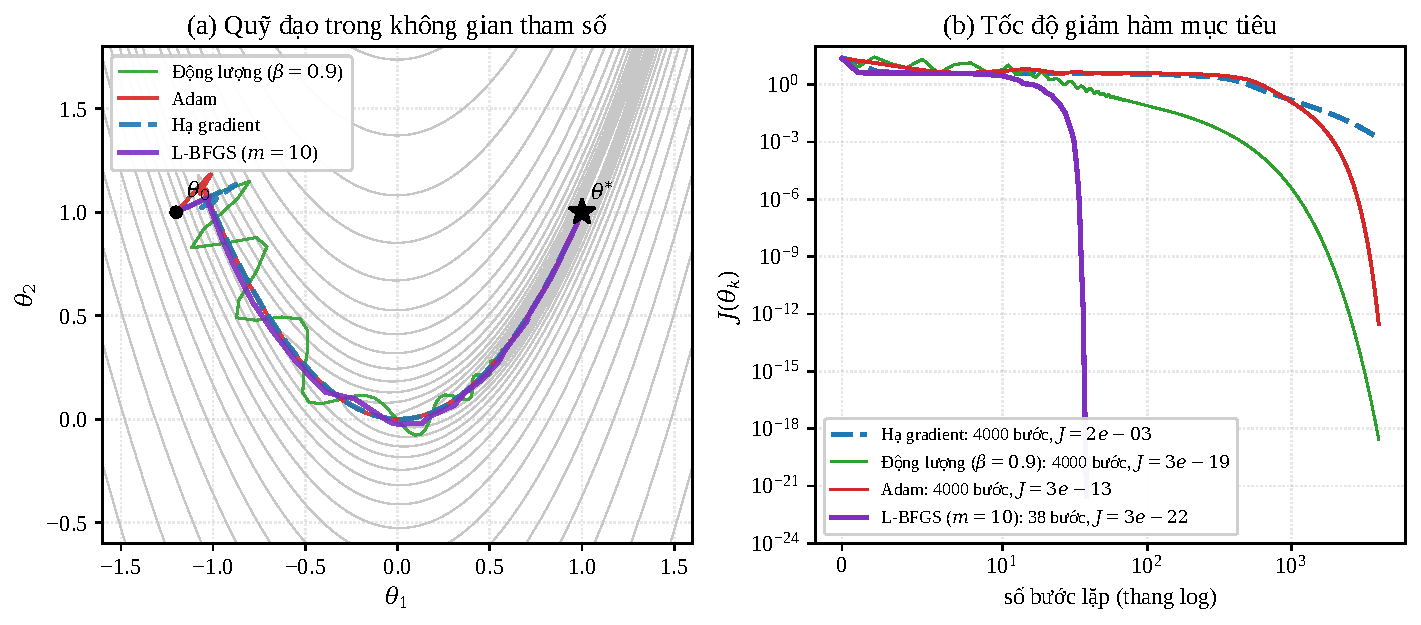
\includegraphics[width=\textwidth]{Images/chap_3/hinh_quydao.pdf}
\caption{So sánh bốn thuật toán tối ưu trên hàm Rosenbrock, cùng điểm xuất phát
$\btheta_0 = (-1{,}2;\,1)$ và cùng nghiệm $\btheta^{\star}=(1;\,1)$. (a) Quỹ đạo
trên nền đường mức; (b) giá trị hàm mục tiêu theo số bước lặp, cả hai trục đều ở
thang lô-ga-rít. Đường L-BFGS dốc đứng ở phía trái phản ánh tốc độ hội tụ siêu
tuyến tính của phương pháp tựa Newton (Nhận xét~\ref{nx:toc-do}).}
\label{fig:quydao}
\end{figure}
 
Cần đọc Hình~\ref{fig:quydao} với một dè dặt: hàm Rosenbrock là hàm hai biến, tất
định, và có nghiệm duy nhất -- không mang ba đặc điểm khó của
Mục~\ref{subsec:dac-thu}. Nó minh hoạ \emph{cơ chế} (thông tin độ cong giúp duỗi
thẳng khe hẹp), không chứng minh điều gì về hàm mục tiêu PINN. Ba lập luận sau
mới là lý do thực chất khiến L-BFGS vượt trội ở giai đoạn cuối trong bối cảnh của
báo cáo.
 
\emph{Thứ nhất, tính tất định.} Trong bài toán PINN, hàm mục tiêu được tính trên
một tập điểm phối trí \emph{cố định}, nên $J(\btheta)$ là hàm tất định và
$\nabla J$ là gradient chính xác chứ không phải ước lượng ngẫu nhiên. Điều kiện
tiên quyết để dùng phương pháp tựa Newton -- các cặp $(\bm{s}_k,\bm{y}_k)$ phản
ánh đúng độ cong -- do đó được thoả mãn. Với gradient nhiễu, hiệu
$\bm{y}_k = \nabla J(\btheta_{k+1}) - \nabla J(\btheta_k)$ là hiệu của hai đại
lượng gần nhau cộng nhiễu, nên phương trình cát tuyến bị bóp méo và xấp xỉ
Hessian nhanh chóng vô nghĩa. Đó là lý do L-BFGS ít được dùng trong học sâu quy
mô lớn với dữ liệu khổng lồ, nhưng lại rất phù hợp ở đây.
 
\emph{Thứ hai, sàn nhiễu.} Theo Mệnh đề~\ref{md:san-nhieu} và
Nhận xét~\ref{nx:noise-floor}, Adam với bước học hằng số chỉ tiệm cận tới một lân
cận của điểm dừng, với mức sàn tỉ lệ tuyến tính theo $\alpha$. Muốn giảm sai số
thêm một bậc, phải giảm bước học một bậc, và tốc độ tiến triển chậm dần tương
ứng. Ngược lại, L-BFGS với tìm kiếm đường Wolfe không có sàn như vậy: nó tiếp tục
giảm $J$ cho tới khi gặp giới hạn của chính số học dấu phẩy động.
 
\emph{Thứ ba, điều kiện xấu.} Hàm mục tiêu \eqref{eq:pinn-loss} là tổng có trọng
của nhiều thành phần có thang độ khác nhau, tạo ra một Hessian có số điều kiện
lớn với các hướng riêng không song song với hệ trục toạ độ. Theo
Nhận xét~\ref{nx:adam-duong-cheo}, xấp xỉ đường chéo của Adam bất lực trước cấu
trúc này, trong khi $\bm{H}_k$ đầy của L-BFGS nắm bắt được tương quan giữa các
toạ độ.
 
Điều ngược lại cũng đúng ở giai đoạn đầu. Khi $\btheta_0$ còn xa nghiệm, mô hình
bậc hai không đáng tin, giả thiết lồi mạnh địa phương của
Nhận xét~\ref{nx:toc-do} không thoả, tìm kiếm đường tốn nhiều lần đánh giá hàm,
và L-BFGS dễ lao thẳng vào cực tiểu địa phương gần nhất -- mà theo
Nhận xét~\ref{nx:doi-xung-hoan-vi}, số lượng cực tiểu như vậy là khổng lồ. Nhiễu
ngẫu nhiên của Adam khi đó lại là một ưu điểm, giúp thoát khỏi các vùng phẳng và
cực tiểu nông.
 
Từ hai nhận định đối lập này, chiến lược chuẩn -- và cũng là chiến lược sẽ áp
dụng ở Chương~\ref{chap:thucnghiem} -- là \emph{huấn luyện hai giai đoạn}.
 
\begin{algorithm}[htbp]
\caption{Chiến lược huấn luyện hai giai đoạn Adam $\to$ L-BFGS}
\label{alg:two-stage}
\begin{algorithmic}[1]
\Require Tham số khởi tạo $\btheta_0$ theo Xavier \eqref{eq:xavier}, số
  vòng $K_{\text{Adam}}$, ngưỡng $\tau$, bộ nhớ $m$
\State \textbf{Giai đoạn 1 (thăm dò).} Chạy Adam
  (Thuật toán~\ref{alg:adam}) với $\alpha = 10^{-3}$ trong $K_{\text{Adam}}$
  vòng lặp, thu $\btheta^{\dagger}$
\State \textbf{Giai đoạn 2 (tinh chỉnh).} Khởi động L-BFGS từ
  $\btheta^{\dagger}$ với tìm kiếm đường Wolfe
  \eqref{eq:wolfe1}--\eqref{eq:wolfe2}, bộ nhớ $m$
\State Dừng khi $\|\nabla J\| < \tau$ hoặc khi tìm kiếm đường thất bại
\State \Return $\btheta^{\star}$
\end{algorithmic}
\end{algorithm}
 
Giai đoạn Adam đưa tham số vào đúng lòng chảo hút của một nghiệm tốt; giai đoạn
L-BFGS khai thác thông tin độ cong để hạ sai số xuống mức mà một bộ giải số
truyền thống có thể so sánh được. Điểm chuyển giao $K_{\text{Adam}}$ là siêu tham
số duy nhất thực sự cần cân nhắc của phác đồ: quá sớm thì L-BFGS chưa ở trong
lòng chảo, quá muộn thì lãng phí vòng lặp ở vùng sàn nhiễu.
 
Hiệu quả của phác đồ được kiểm chứng ở Hình~\ref{fig:hoitu} trên một bài toán
khớp hàm mẫu $u(x)=\sin(3x)\,e^{-x^2/2}$ bằng mạng $(1,16,16,1)$ với hàm kích
hoạt $\tanh$, khởi tạo Xavier, dùng $201$ điểm phân bố đều trên $[-3,3]$. Cài đặt
hoàn toàn bằng NumPy với lan truyền ngược viết tay theo đúng
\eqref{eq:bp1}--\eqref{eq:bp4}, nên hình vẽ phản ánh chính xác lý thuyết đã trình
bày chứ không phải hành vi của một thư viện. Kết quả rõ rệt: Adam chạy đơn thuần
$20\,000$ vòng chững lại ở $J \approx 7{,}7\cdot 10^{-7}$ và dao động quanh mức
đó -- đúng hiện tượng sàn nhiễu của Mệnh đề~\ref{md:san-nhieu} -- trong khi chỉ
cần $2000$ vòng Adam rồi chuyển sang L-BFGS, hàm mục tiêu tiếp tục giảm đều đặn
xuống $J \approx 9{,}1\cdot 10^{-10}$, tốt hơn khoảng $850$ lần với tổng số vòng
lặp tương đương.
 
\begin{figure}[htbp]
\centering
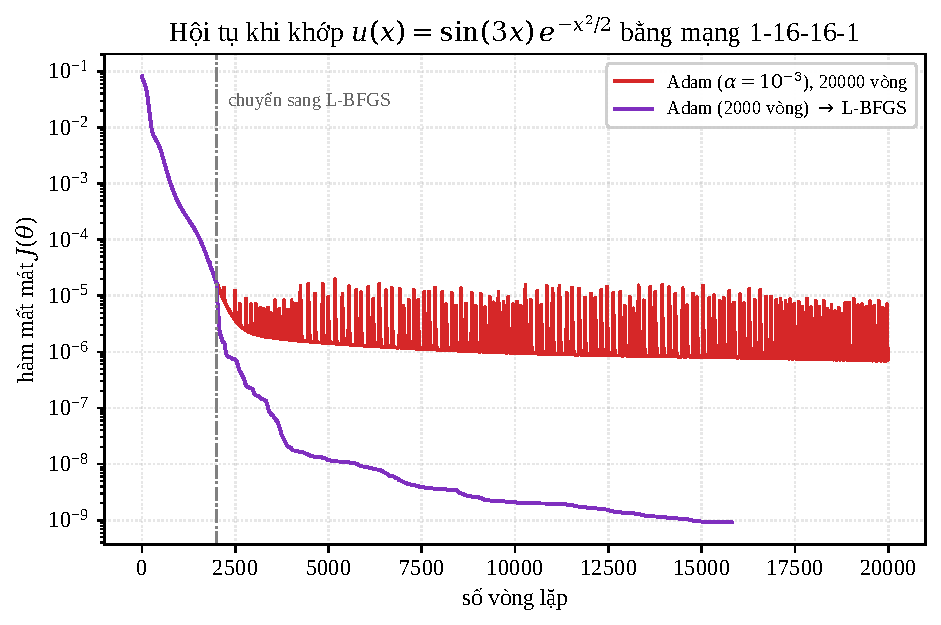
\includegraphics[width=0.86\textwidth]{Images/chap_3/hinh_hoitu.pdf}
\caption{Đường cong hội tụ khi khớp $u(x)=\sin(3x)\,e^{-x^2/2}$ bằng mạng
$(1,16,16,1)$. Đường màu đỏ: Adam với $\alpha=10^{-3}$ chạy liên tục. Đường màu
tím: chiến lược hai giai đoạn, chuyển sang L-BFGS ($m=20$) tại vòng $2000$ (vạch
đứt dọc). Trục tung ở thang lô-ga-rít.}
\label{fig:hoitu}
\end{figure}
 
\begin{nhanxet}[Phạm vi của kết luận]
Thí nghiệm ở Hình~\ref{fig:hoitu} là bài toán \emph{khớp hàm} có nhãn, không phải
bài toán phần dư. Nó kiểm chứng cơ chế sàn nhiễu và lợi ích của giai đoạn tinh
chỉnh trên một hàm mục tiêu tất định, nhưng chưa nói gì về hàm mục tiêu
\eqref{eq:pinn-loss} với nhiều thành phần cạnh tranh. Kết quả định lượng của
chiến lược này trên các bài toán đạo hàm riêng sẽ được trình bày ở
Chương~\ref{chap:thucnghiem}, và cần được đọc như phần kiểm chứng thực sự của
Mục này. Ngoài ra, con số ``$850$ lần'' đến từ một hạt giống ngẫu nhiên; theo
Nhận xét~\ref{nx:doi-xung-hoan-vi}, mọi so sánh giữa hai phác đồ huấn luyện phải
được lặp lại trên nhiều hạt giống trước khi rút kết luận.
\end{nhanxet}
 
%==============================================================================
\section*{Kết luận chương}
\addcontentsline{toc}{section}{Kết luận chương}
%==============================================================================
 
Chương này đã thiết lập bộ công cụ tính toán cho phần còn lại của báo cáo; các
kết quả chính được tổng hợp ở Bảng~\ref{tab:tong-ket-3}.
 
Lan truyền ngược được trình bày như một trường hợp riêng của quy tắc dây chuyền
trên đồ thị tính toán \eqref{eq:chain-graph}, dẫn tới bốn phương trình
\eqref{eq:bp1}--\eqref{eq:bp4} và kết quả then chốt của
Mệnh đề~\ref{md:chi-phi-bp}: chi phí tính gradient chỉ bằng một bội số nhỏ của
chi phí đánh giá hàm, độc lập với số tham số.
 
Vi phân tự động được phân biệt rạch ròi với vi phân ký hiệu và vi phân số.
Mệnh đề~\ref{md:fd-rao-can} chứng minh rằng sai phân hữu hạn bị chặn ở bậc
$\eps^{2/3}$ do xung đột giữa sai số cắt cụt và sai số làm tròn, và
Bảng~\ref{tab:fd-error} xác nhận cả hai nhánh tiệm cận. Quan trọng hơn,
Mệnh đề~\ref{md:ad-tai-tao} khép lại mắt xích còn để ngỏ ở cuối
Chương~\ref{chap:fnn}: cơ chế thuận-trên-thuận của vi phân tự động tái tạo
\emph{đúng} hai hệ thức truy hồi \eqref{eq:G-truy-hoi} và \eqref{eq:S-truy-hoi},
mà không đòi hỏi lập trình tường minh $\sigma''$.
 
Về tối ưu hoá, hai thuật toán đại diện cho hai triết lý đã được phân tích cùng
với chứng minh cho những khẳng định mà tài liệu thường chỉ nêu định tính: sàn
nhiễu của bước học hằng số (Mệnh đề~\ref{md:san-nhieu}), hệ số khuếch đại
$1/(1-\beta)$ của động lượng (Bổ đề~\ref{bd:momentum}), tính cần thiết của hiệu
chỉnh độ chệch trong Adam (Bổ đề~\ref{bd:adam-bias}), và việc điều kiện Wolfe kéo
theo điều kiện độ cong (Bổ đề~\ref{bd:wolfe-curvature}). Chiến lược hai giai đoạn
Adam $\to$ L-BFGS được biện minh bằng ba lập luận -- tính tất định của gradient,
sàn nhiễu, và điều kiện xấu -- chứ không bằng kinh nghiệm thực hành.
 
\begin{table}[htbp]
\centering
\caption{Tổng kết các kết quả chính của Chương~\ref{chap:autodiff}.}
\label{tab:tong-ket-3}
\small
\begin{tabular}{@{}l p{8.2cm}@{}}
\toprule
\textbf{Kết quả} & \textbf{Nội dung và vai trò} \\
\midrule
Mệnh đề~\ref{md:bp}
  & Bốn phương trình lan truyền ngược cho mạng lớp ra tuyến tính; dạng lô
    \eqref{eq:bp-batch}. \\
Mệnh đề~\ref{md:chi-phi-bp}
  & $\mathrm{cost}(\nabla_{\btheta}J) \le 3\,\mathrm{cost}(J)$, độc lập $P$;
    trường hợp riêng có hằng số cụ thể của Định lý~\ref{dl:cheap-gradient}. \\
Mệnh đề~\ref{md:fd-rao-can}
  & Sai phân trung tâm có đáy sai số bậc $\eps^{2/3}$ tại
    $h^{*}\sim\eps^{1/3}$; hằng số phụ thuộc bài toán
    (Nhận xét~\ref{nx:fd-hang-so}). \\
Bổ đề~\ref{bd:doi-ngau}
  & Số đối ngẫu: $f(a+b\epsilon) = f(a)+f'(a)b\epsilon$ -- nguyên lý của chế độ
    thuận. \\
Định lý~\ref{dl:cheap-gradient}
  & Nguyên lý gradient rẻ: hằng số không phụ thuộc số biến. \\
\textbf{Mệnh đề~\ref{md:ad-tai-tao}}
  & \textbf{Vi phân tự động tái tạo đúng các truy hồi
    \eqref{eq:G-truy-hoi}, \eqref{eq:S-truy-hoi} của Chương~\ref{chap:fnn}};
    mỗi lượt cho một dạng toàn phương của Hessian. \\
Mệnh đề~\ref{md:san-nhieu}
  & Sàn nhiễu: $\E[J] \to \alpha\varsigma^2/\big(2(2-\alpha\mu)\big)$, tuyến
    tính theo bước học. \\
Bổ đề~\ref{bd:momentum}
  & Động lượng khuếch đại thành phần nhất quán $1/(1-\beta)$ lần và nén thành
    phần dao động $1/(1+\beta)$ lần. \\
Bổ đề~\ref{bd:adam-bias}
  & $\E[\bm{m}_k] = (1-\beta_1^k)\bm{g}$: hiệu chỉnh độ chệch là cần thiết ở
    các bước đầu. \\
Bổ đề~\ref{bd:wolfe-curvature}
  & Điều kiện Wolfe kéo theo $\bm{y}_k^{\top}\bm{s}_k > 0$, bảo toàn tính xác
    định dương của $\bm{H}_k$. \\
Mệnh đề~\ref{md:two-loop-cost}
  & Đệ quy hai vòng: $\mathcal{O}(mP)$ thời gian và bộ nhớ, không dựng
    $\bm{H}_k$. \\
\bottomrule
\end{tabular}
\end{table}
 
Với nền tảng này, Chương~\ref{chap:pinn} có thể tập trung vào nội dung riêng của
phương pháp: cách xây dựng hàm mục tiêu từ phần dư phương trình vi phân, cách áp
đặt điều kiện đầu và điều kiện biên -- hoặc bằng ràng buộc mềm qua trọng số
$\lambda$ trong \eqref{eq:pinn-loss}, hoặc bằng ràng buộc cứng qua nghiệm thử --
và các đặc tính hội tụ của mạng nơ-ron thông tin vật lý.
 